% =====================================================================
%  博士科研计划书 —— 面向聚变堆复杂几何的体素化特征线中子输运与GPU并行加速方法研究
%  版本：V2.1（完整五章修订）（2026-11-11）
%  编译：xelatex main.tex  ×3（生成目录与交叉引用）
% =====================================================================
\documentclass[UTF8, zihao=-4, fontset=none, a4paper]{ctexart}

\usepackage{fontspec}
\setmainfont{Times New Roman}
\setsansfont{Helvetica}
\setCJKmainfont{Songti SC}[AutoFakeBold=2.2, AutoFakeSlant=0.2]
\setCJKsansfont{Heiti SC}[AutoFakeBold=2.2]
\setCJKmonofont{Songti SC}
\newCJKfontfamily\songti{Songti SC}
\newCJKfontfamily\heiti{Heiti SC}
\newCJKfontfamily\fangsong{Songti SC}
\newCJKfontfamily\kaishu{Songti SC}

\usepackage[a4paper, top=2.6cm, bottom=2.6cm, left=2.7cm, right=2.7cm]{geometry}
\usepackage{amsmath, amssymb}
\usepackage{graphicx}
\usepackage{booktabs}
\usepackage{longtable}
\usepackage{etoolbox}
\usepackage{needspace}
\usepackage{array}
\usepackage{calc}
\usepackage{caption}
\usepackage{fancyhdr}
\usepackage{enumitem}
\usepackage[hidelinks, bookmarksnumbered, bookmarksopen]{hyperref}

% ---------------- 版式 ----------------
\linespread{1.42}
\setlength{\parskip}{0.35em}
\setlength{\parindent}{2em}

\pagestyle{fancy}
\fancyhf{}
\fancyfoot[C]{\zihao{-5}\thepage}
\renewcommand{\headrulewidth}{0pt}

% 章标题：第一章 / 节标题：1.1 （自动编号，与原文手工编号一致）
\ctexset{
  section = {
    name       = {第,章},
    number     = \chinese{section},
    format     = \centering\zihao{3}\bfseries,
    beforeskip = 1.2ex plus .2ex,
    afterskip  = 2.2ex plus .2ex,
  },
  subsection = {
    format     = \zihao{4}\bfseries,
    beforeskip = 1.8ex plus .3ex,
    afterskip  = 1.0ex plus .2ex,
  },
}
\renewcommand{\thesubsection}{\arabic{section}.\arabic{subsection}}

% 图表标题
\captionsetup{font=small, labelsep=quad, skip=6pt}
\captionsetup[longtable]{font=small, labelsep=quad, skip=4pt}
\AtBeginEnvironment{longtable}{\small}

% ---------------- 自定义命令 ----------------
% 上标数字引文，例如 \upcite{1,2} -> [1,2]
\newcommand{\upcite}[1]{\textsuperscript{[#1]}}

\graphicspath{{figures/}}
\hypersetup{pdfinfo={FigureSources={ARIES project official CAD library, Cross-Section and 3D Sector; Yang, Yang, Popov and Buchan (2025), DOI 10.3389/fnuen.2025.1597165, Figure 1(b,d), selected and rearranged, CC BY 4.0 https://creativecommons.org/licenses/by/4.0/}}}

% =====================================================================

% Chapter summaries and comparison tables share 10.5 pt text and captions.
\DeclareCaptionFont{tabletext}{\fontsize{10.5}{14}\selectfont}
\captionsetup[table]{font=tabletext,labelsep=quad}
\newcommand{\SummaryTable}[3]{%
\par\addvspace{6pt}\noindent\begin{minipage}{\linewidth}\fontsize{10.5}{15}\selectfont
\setlength{\tabcolsep}{5pt}\renewcommand{\arraystretch}{1.2}
\captionof{table}{#1}\label{#2}\par
\begin{tabular}{@{}>{\raggedright\arraybackslash}p{\dimexpr.18\linewidth-1.34\tabcolsep\relax}>{\raggedright\arraybackslash}p{\dimexpr.40\linewidth-1.33\tabcolsep\relax}>{\raggedright\arraybackslash}p{\dimexpr.42\linewidth-1.33\tabcolsep\relax}@{}}
\toprule
#3\bottomrule
\end{tabular}\end{minipage}\par\addvspace{6pt}}

\begin{document}

% ---------------- 封面 ----------------
\begin{titlepage}
  \centering
  \vspace*{2.4cm}
  {\zihao{2}\bfseries 博士生科研计划书\par}
  \vspace{2.2cm}
  \begin{minipage}{0.9\linewidth}
    \zihao{4}
    \renewcommand{\arraystretch}{1.9}
    \begin{tabular}{@{}>{\raggedright\arraybackslash}p{5em}>{\raggedright\arraybackslash}p{\dimexpr\linewidth-5em-2\tabcolsep\relax}@{}}
      学生姓名： & 周璐楠 \\
      报考院系： & 机械与动力工程学院 \\
      报考专业： & 核科学与技术 \\
      研究方向： & 反应堆物理 \\
      导师： & 张滕飞 \\
      论文题目： & 面向聚变堆复杂几何的体素化特征线中子输运与GPU并行加速方法研究
    \end{tabular}
  \end{minipage}
  \vfill
  {\zihao{5} 2026 年 11 月 11 日\par}
  \vspace*{1cm}
\end{titlepage}

% ---------------- 目录 ----------------
\pagenumbering{roman}
\begingroup
\linespread{1.05}\selectfont
\setlength{\parskip}{0pt}
\tableofcontents
\endgroup
\clearpage

% ---------------- 正文 ----------------
\pagenumbering{arabic}
\setcounter{page}{1}




\section{研究背景与研究目标}\label{sec:1}
\subsection{聚变堆中子屏蔽的工程需求与计算挑战}
D-T聚变中子产生于真空室内的等离子体，初始能量约为14 MeV。中子向外传播，穿过第一壁、包层、真空室壁及屏蔽体等结构，在材料中发生散射、吸收，并产生次级中子和光子，形成包含高能中子及慢化中子的辐射场。屏蔽设计需在装置空间与材料约束下，控制屏蔽体外的中子通量及相应反应率。现有聚变中子学研究已将三维几何建模、输运求解与设计方案比较结合起来\upcite{1,2}。本研究以中子能谱、区域通量和指定反应率为主要评价量，研究复杂屏蔽结构中的中子输运计算。

聚变装置的几何复杂性不仅表现为部件数量多，还表现为材料界面和传播通道对输运结果的影响。图\ref{fig:aries}所示的ARIES-RS概念设计中，包层、屏蔽层和真空室呈分层嵌套布置，同时包含为检修和更换设置的部件分段、支承及集管等结构\upcite{3}。多层材料决定中子依次经历的碰撞和能谱变化；薄壁和斜交界面的几何近似会改变射线穿过各材料的长度；诊断孔道及管线穿透件可能为中子提供穿过较少屏蔽材料的传播通道。一条窄通道是否贯通，就可能改变其在屏蔽体外对应位置的中子通量和能谱。
\begin{figure}[htbp]
\centering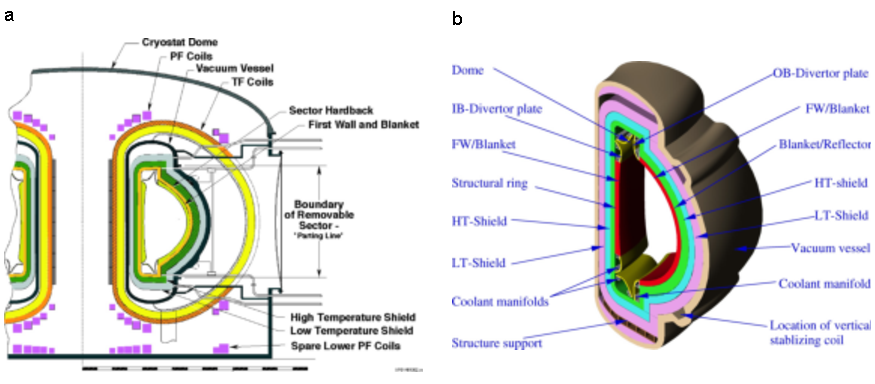
\includegraphics[width=0.95\linewidth]{figures/aries_rs}
\caption{ARIES-RS整体剖面与包层—屏蔽扇区\upcite{3}}\label{fig:aries}
\end{figure}

这类问题同时要求精度与效率。几何结构改变后，需要更新材料分布及相应的材料路径。材料组成或密度改变时，需要更新相应截面。三维输运计算需要同时处理空间、能量和传播方向上的变化，计算量随空间单元数、离散方向数、能群数及迭代次数增加。全域细网格会增加轨迹分段数、源区数量及通量数组的存储需求，简化材料界面和孔道会改变孔道连通性及中子穿过各层材料的长度。研究需要确定应保留哪些影响中子能谱、区域通量和指定反应率的几何信息，并在有限资源下完成相应的输运计算。

\subsection{中子输运数值方法及 MOC 的选择依据}
采用三维、稳态、多群固定源模型，将中子能量划分为$G$个能群，外源已知。对空间位置$\mathbf r$、单位方向向量$\Omega$和能群$g=1,\ldots,G$，输运方程写为
\begin{equation}
\Omega\cdot\nabla\psi_g(\mathbf r,\Omega)+\Sigma_{t,g}(\mathbf r)\psi_g(\mathbf r,\Omega)
=q_g(\mathbf r,\Omega)+\sum_{g'=1}^{G}\int_{4\pi}K_{g'\to g}(\mathbf r,\Omega'\to\Omega)\psi_{g'}(\mathbf r,\Omega')\,d\Omega'.
\label{eq:transport}
\end{equation}
式中$\psi_g(\mathbf r,\Omega)$为第$g$群角通量，由能量相关角通量在该群能区内积分得到；$\Sigma_{t,g}(\mathbf r)$为第$g$群宏观总截面；$q_g(\mathbf r,\Omega)$为已知外源。$K_{g'\to g}$为宏观微分中子转移截面，描述中子由能群$g'$、方向$\Omega'$转移到能群$g$、方向$\Omega$，包括散射及所纳入的$(n,2n)$等反应的中子产生贡献。对仅依赖散射角余弦$\mu_0=\Omega'\cdot\Omega$的角分布，采用勒让德展开
\begin{equation}
K_{g'\to g}(\mathbf r,\mu_0)\simeq
\sum_{l=0}^{L}\frac{2l+1}{4\pi}K_{l,g'\to g}(\mathbf r)P_l(\mu_0).
\label{eq:legendre}
\end{equation}
$P_l$为$l$阶勒让德多项式，$K_{l,g'\to g}$为相应转移截面矩，$L$为截断阶。记计算区域外表面为$S$、外法向单位向量为$\mathbf n$，真空边界条件为
\begin{equation}
\psi_g(\mathbf r,\Omega)=0,\qquad \mathbf r\in S,\quad \Omega\cdot\mathbf n<0.
\label{eq:vacuum}
\end{equation}

第$g$群标量通量是角通量对全立体角的积分。区域$V_d$上的响应取标量通量的线性泛函，
\begin{equation}
\phi_g(\mathbf r)=\int_{4\pi}\psi_g(\mathbf r,\Omega)\,d\Omega,\qquad
R_d=\sum_{g=1}^{G}\int_{V_d}d_{d,g}(\mathbf r)\phi_g(\mathbf r)\,dV.
\label{eq:response}
\end{equation}
权重$d_{d,g}$按所求量选取。第$g_0$群的区域平均通量、反应$x$的区域总反应率及中子周围剂量当量率分别定义为
\begin{equation}
\begin{aligned}
\overline\phi_{d,g_0}&=\frac{1}{|V_d|}\int_{V_d}\phi_{g_0}(\mathbf r)\,dV,
&&d_{d,g}=\frac{\delta_{gg_0}}{|V_d|},\\
R_{x,d}&=\sum_{g=1}^{G}\int_{V_d}\Sigma_{x,g}(\mathbf r)\phi_g(\mathbf r)\,dV,
&&d_{d,g}=\Sigma_{x,g},\\
\overline{\dot H^*(10)}_d&=\frac{1}{|V_d|}\sum_{g=1}^{G}\int_{V_d}f_g\phi_g(\mathbf r)\,dV,
&&d_{d,g}=\frac{f_g}{|V_d|}.
\end{aligned}
\label{eq:response_examples}
\end{equation}
其中$\delta_{gg_0}$为克罗内克符号，$\Sigma_{x,g}$为指定反应的群宏观截面。$f_g$为第$g$群的中子注量—周围剂量当量转换系数，由ICRP 74的能量相关转换系数按群内中子谱加权得到\upcite{4}。$\overline{\dot H^*(10)}_d$表示区域平均中子周围剂量当量率。

屏蔽体外的通量和能谱取决于中子传播中经历的材料分层、各层厚度，以及孔道或缝隙是否贯通。蒙特卡罗方法（MC）、离散纵标方法（$S_N$）和特征线方法（MOC）处理这些几何信息及空间、角度积分的方式不同。MC通过抽样粒子飞行和碰撞历史估计响应，能够处理连续能量和复杂几何，结果具有统计误差。深穿透条件下，对远端计分有贡献的历史较少，通量和能谱估计通常需要较多源历史或减方差技术。$S_N$在有限离散方向上求解输运方程，采用差分或有限元等方法进行空间离散，材料界面由网格边界或单元内的材料分布表示。MOC同样采用离散方向，但沿射线穿过的材料段计算角通量，再用轨迹和角向求积得到源区通量。两种确定论方法均需检验空间与角向收敛，孔道流束的计算尤其依赖离散方向与孔道轴向的相对关系。

OpenMOC采用平源近似和源迭代\upcite{5}，三维非结构网格MOC研究实现了长特征线输运求解\upcite{6}。对给定能群、离散方向和源迭代步，将散射、次级中子产生与外源构成的总角源简记为$Q$。段内宏观总截面$\Sigma_t$和$Q$均为常数、且$\Sigma_t>0$时，出射角通量为
\begin{equation}
\psi_{\rm out}=\psi_{\rm in}e^{-\Sigma_t\ell}
+\frac{Q}{\Sigma_t}\left(1-e^{-\Sigma_t\ell}\right).
\label{eq:moc_out}
\end{equation}
$\ell$为该段长度，$\psi_{\rm in}$为入射角通量。$\Sigma_t\to0$时，上式取极限$\psi_{\rm out}=\psi_{\rm in}+Q\ell$。前一段的出射角通量是下一段的入射角通量，各段衰减和源贡献随路径传递，材料截面及段长偏差因而可能影响屏蔽体外的通量和能谱。

采用MOC的依据在于材料路径与段内输运计算之间的直接联系。材料次序和段长确定后，式\eqref{eq:moc_out}将入射角通量、材料衰减和段内总源的积分联系起来。段长与截面的变化通过材料段角通量计算，影响标量通量及反应率。对于散射问题，根据上一轮通量更新散射源后，继续扫描同一组轨迹，直至源迭代收敛。

三维MOC的主要计算量随轨迹数、段数、能群数和扫描轮数增长。固定几何的段数据可在能群与源迭代间复用，不同完整轨迹又可并行扫描。体素化后，通过单元索引读取材料编号，并沿射线逐单元计算材料段长，GPU执行则围绕这些材料段安排扫描和通量求和。因此，本研究考察体素材料界面对输运精度的影响、局部细化增加的轨迹计算量，以及GPU执行效率。

\subsection{复杂几何体素化与 GPU 异构并行技术路线}
MOC需要确定每条射线依次穿过的材料及其段长。直接几何追踪通过计算射线与CAD/CSG边界的交点取得这些区间，曲面求交和材料定位构成轨迹生成的重要工作。

体素化先将原几何映射为规则网格上的材料分布。在覆盖计算区域的长方体内划分笛卡尔单元，每个基础体素记录一种材料编号。射线进入网格后依次穿过单元，由入射点和出射点确定单元内的段长，再按单元索引读取材料，无需逐次查询原CAD曲面。同一材料网格可供不同方向、能群和源迭代使用，各条射线的穿越区间仍由其位置和方向确定。薄层、斜交界面和孔道附近的单元局部细化，其余区域保持较粗，能够避免全域使用同等细网格。

笛卡尔体素面通常不与真实材料界面重合，射线进入或离开某种材料的位置因而发生偏移，材料段长甚至材料次序可能改变。窄孔道可能被周围材料封闭，薄壁也可能未被网格保留，从而形成原几何中不存在的缝隙。局部细化可减小上述几何偏差。细化还会增加轨迹子段、源区及更新工作量，使网格分辨率同时影响响应误差和计算成本。

三维特征线扫描对大量材料段执行相同形式的角通量计算，适合GPU并行处理。轨迹之间的段数差异、同一源区的并发求和及显存容量共同影响扫描效率。已有GPU-MOC工作采用在线分段和轨迹分批处理，协调段数据存储与扫描任务\upcite{7,8}。轨迹分批处理是将轨迹分批传入GPU显存，每批完成扫描和通量累加后，再处理下一批。

技术路线以规则体素和局部层级细化表示材料，以三维多群MOC求解输运，结合CPU与GPU的任务划分开展GPU异构并行研究。数值误差和计算工作量共同决定网格分辨率与执行参数的选择。

\subsection{研究目标与关键科学问题}
面向多层材料与复杂孔道屏蔽，本研究以体素化三维MOC为基础，开展材料路径误差与响应精度控制、GPU异构并行，以及精度和显存约束下的参数选择研究。围绕这一目标提出三个研究问题。

\textbf{问题一：体素化MOC的数值精度。}体素界面与真实材料界面不一致时，材料路径和光学厚度发生偏差。这些偏差在深穿透条件下如何影响屏蔽体外的通量、能谱和反应率？能否结合射线经过的材料次序和段长、正向通量及伴随通量估计目标响应偏差，并识别需要局部细化的位置？如何同时控制几何映射与MOC输运离散误差？

\textbf{问题二：GPU上的轨迹扫描。}局部细化和材料分布不均会改变各轨迹的材料段数与数据访问量。在显存限制下，如何安排材料段缓存、轨迹任务和源区通量求和，减少重复计算与线程等待，缩短完整求解时间？

\textbf{问题三：精度与成本的协同选择。}真实误差事先未知，如何利用可计算的误差指标与少量试算，预测响应误差、运行时间和GPU峰值显存，选择体素尺寸、源区划分及GPU执行参数，使指定响应误差容限与显存约束下的完整计算成本尽可能低？

输运模型采用稳态、多群中子固定源，几何采用规则体素及局部层级细化，计算由CPU与GPU协同完成。通过射线与原CAD/CSG边界求交获得参考材料段，核对体素追踪得到的材料次序和段长。程序以二维均匀体素网格上的CPU计算为起点，通过与解析解比较验证数值结果，再扩展至三维体素、GPU扫描、伴随求解和局部细化。验证包括多层材料屏蔽与孔道流束算例，并通过与独立程序计算结果和实验数据比较，检验区域通量、指定反应率及中子能谱的计算结果，结合参考计算与实验不确定度解释差异。

\section{复杂几何体素化与 MOC 数值方法研究现状}\label{sec:2}
\subsection{复杂几何表示与材料映射方法}
输运计算中的几何表示需要回答两个问题：中子位于哪种材料，以及沿给定方向何时进入下一种材料。MOC还需沿整条射线取得有序材料段及其长度。因此，几何转换既要形成材料明确、无遗漏和无重叠的分区，也要能够生成可靠的材料路径。表\ref{tab:geometry_compare}比较五类几何处理方式如何确定材料段、重复扫描时读取或重建哪些数据，以及如何表示材料界面。

CAD用曲面和实体描述部件，CSG用基本曲面和布尔运算定义区域。McCad的ITER转换研究将CAD整理为输运几何，并用MCNP随机体积估计与CAD体积比较，检查材料区域的转换偏差\upcite{9}。Chen等在SuperMC中对CAD边界求交，以交点确定材料段，说明直接几何访问能够用于二维MOC分段\upcite{10}。

面元化边界把曲面分成三角面。确定粒子下一次碰到哪张面时，需要将飞行射线与三角面求交。面元很多时，频繁求交会增加几何查询时间。Shriwise等在DAGMC中用有符号距离场估计当前位置到最近表面的距离，并结合插值误差界判断是否需要求交\upcite{11}。例如，若计划飞行距离小于距离估计扣除误差界后的保守下界，就能确定这一步不会穿越表面，从而跳过求交。不能排除穿越可能时，仍按原来的三角面追踪计算。基于Embree的后续工作则减少必须求交时的计算量\upcite{12}。这些方法节省的是蒙特卡罗输运中单步表面查询的时间。特征线法需要从入射到出射的完整材料段，包括每段的长度、材料编号和先后次序。这些数据可以在首次追踪后保存，供后续扫描读取，也可以在每次扫描时重新生成。两种做法的存储量和重复计算量不同，完整扫描的计算时间还取决于材料段的生成与读取方式。

非贴体网格不要求单元边界与材料界面重合，材料界面可以穿过背景单元。Yang等把边界表示转换为构造实体几何（CSG），再按单元内各材料所占的体积分数构造均匀化材料，整个单元使用同一组宏观截面\upcite{13}。Buchan等把实体网格与背景网格的重叠部分用于守恒投影，并让背景网格在需要的位置加密\upcite{14}。这些处理保留单元或投影区域内各材料的体积占比，却不能据此确定沿射线遇到材料的次序及各材料段的长度。相同的空隙比例既可以连成贯通孔道，也可以分成若干封闭空腔。孔道贯通时，中子可以在空隙中飞行较长距离。体积均匀化用等效宏观截面代替单元内部的材料分布，中子沿贯通孔道穿过该单元时，原本位于空隙中的行程也被赋予非零碰撞截面，因而高估这一路径上的碰撞概率。

另一类方法移动材料界面附近的网格节点，使单元边界贴合材料界面，远离界面的区域保留规则网格。Liang Yang等的体素主导网格采用这种局部调整，图\ref{fig:mesh}比较阶梯边界与贴合边界\upcite{15}。
\begin{figure}[htbp]
\centering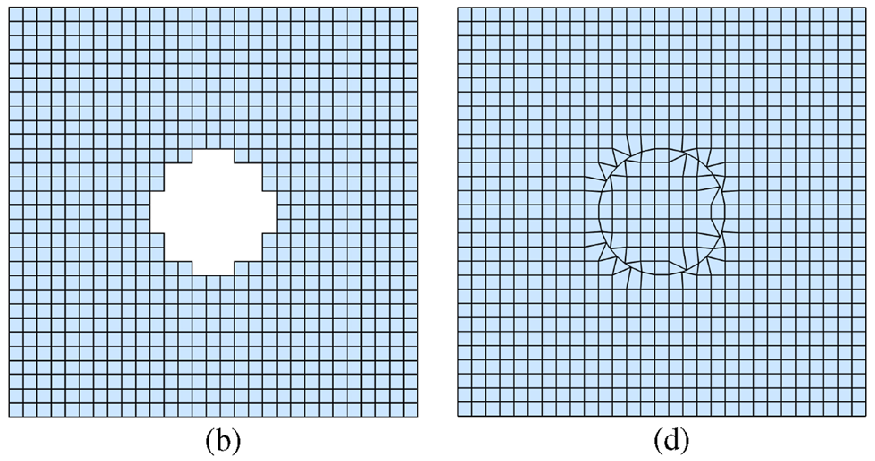
\includegraphics[width=0.5\linewidth]{figures/yang_mesh}
\caption{阶梯边界与边界贴合的体素主导网格\upcite{15}}\label{fig:mesh}
\end{figure}

规则体素直接保存单元材料编号，固定材料场可供不同方向和源迭代重复访问。中心点赋材按体素中心所在的材料，为整个体素指定材料编号。单元内多点采样则根据各材料所占的采样点比例，估计材料体积分数。局部细化采用更小的体素表示材料界面、薄层和孔道。Liu等在多层八叉树上处理不同尺寸的非匹配笛卡尔单元，用于$S_N$输运\upcite{16}。AMReX将局部细网格组织为规则网格块，保存各块上的单元数据，并在细化区域改变时重建网格块及更新相应数据\upcite{17}。

\Needspace{10\baselineskip}
\begingroup
\fontsize{10.5}{15}\selectfont
\setlength{\tabcolsep}{4pt}\renewcommand{\arraystretch}{1.18}
\begin{longtable}{@{}>{\raggedright\arraybackslash}p{\dimexpr.16\linewidth-1.6\tabcolsep\relax}>{\raggedright\arraybackslash}p{\dimexpr.23\linewidth-1.6\tabcolsep\relax}>{\raggedright\arraybackslash}p{\dimexpr.22\linewidth-1.6\tabcolsep\relax}>{\raggedright\arraybackslash}p{\dimexpr.23\linewidth-1.6\tabcolsep\relax}>{\raggedright\arraybackslash}p{\dimexpr.16\linewidth-1.6\tabcolsep\relax}@{}}
\caption{几何处理方式的材料分段与重复扫描}\label{tab:geometry_compare}\\
\toprule
几何处理 & 材料段的确定 & 重复扫描与几何更新 & 材料界面与孔道的表示 & 代表工作\\\midrule
\endfirsthead
\multicolumn{5}{c}{表\thetable\ （续）}\\\toprule
几何处理 & 材料段的确定 & 重复扫描与几何更新 & 材料界面与孔道的表示 & 代表工作\\\midrule
\endhead
\bottomrule\endlastfoot
CAD/CSG直接求交 & 曲面交点确定段长和材料 & 保存后供各能群和源迭代读取，几何或轨迹改变时重建 & 以CAD曲面或CSG曲面表示材料边界 & McCad\upcite{9}、SuperMC\upcite{10}\\
面元边界与辅助距离场 & 面元求交，距离场保守预筛选 & 保存材料段后读取，重新生成时用距离场减少求交 & 以三角面元近似曲面，距离场用于筛选求交 & DAGMC\upcite{11,12}\\
体积分数投影 & 按体积分数构造单元混合材料 & 读取投影后的单元材料数据，几何或材料改变时重新投影 & 以单元混合材料表示材料占比 & Yang\upcite{13}、Buchan\upcite{14}\\
界面节点调整 & 调整界面单元，再按单元边界分段 & 读取已生成的段，界面改变时调整局部节点并重新分段 & 以调整后的单元边界贴合材料界面 & Liang Yang\upcite{15}\\
规则体素与层级块 & 按单元索引读取材料，沿射线逐单元确定段长 & 读取单元材料数据，局部细化后重新确定受影响的材料段 & 以体素边界表示材料界面与孔道形状 & Liu\upcite{16}、AMReX\upcite{17}\\
\end{longtable}
\endgroup

\subsection{体素化几何与 MOC 特征线离散的耦合}
几何模型确定材料区域，特征线追踪计算射线在各区域内的段长，特征线离散同时确定用于空间和角向积分的轨迹及权重。三维长特征线研究已将轨迹与非结构源区关联，模块化追踪则利用重复几何保存局部段序列，减少重复构建\upcite{6,18}。

规则网格中的段长是射线进入和离开当前单元的两个交点之间的距离。Amanatides–Woo遍历分别记录射线与下一处$x$、$y$、$z$方向网格面的交点参数，每次推进到最近的交点，更新单元编号及该方向的下一交点参数\upcite{19}。射线同时穿过网格棱或顶点时，同步更新相应的两个或三个坐标索引。层级网格中不再继续细分的单元称为叶单元。不同叶单元的尺寸可以不同，射线跨越粗细网格交界时，需要定位下一个单元并重新计算出射位置。Laine与Karras用稀疏八叉树存储体素，并通过层级遍历查找射线经过的叶单元\upcite{20}。中子输运追踪需记录射线穿过材料区和真空区的全部区间。

将材料区与源项近似区域的交叠区域定义为实际计算源区，以下统一记为$r$。每段除了长度，还需关联材料、源区和计分区。材料编号决定截面，源区决定源项近似，计分区决定响应积分。射线穿过材料界面、源区边界或计分区边界时，应在交点处分段。需要计算粗网界面中子流时，也在相应交点处分段。各子段使用对应的材料截面和源项逐段计算角通量，段积分计入相应源区和计分区，穿越粗网界面的角通量用于计算界面中子流。式\eqref{eq:moc_out}的形式不因追踪方式改变，但其中的截面、段长和段内源由分段数据提供。

方向$\Omega_n$及角权重$w_n$离散角积分，满足$\sum_nw_n=4\pi$。垂直于该方向布置的轨迹$k$以横截面面积权重$a_{kn}$代表射线束。对源区$r$，空间求积应满足
\begin{equation}
V_{r,n}^{\rm tr}=\sum_{(k,s)\in r}a_{kn}\ell_{kns}\simeq V_r.
\label{eq:volume}
\end{equation}
$s$为轨迹子段，$\ell_{kns}$为其长度，$V_r$为既定离散模型的源区体积。$V_{r,n}^{\rm tr}$与$V_r$的差反映有限轨迹的体积求积和覆盖误差，体素材料体积与原几何体积的差则属于几何映射误差。

局部细化后，重新确定受影响轨迹的分段点、各段长度，以及对应的材料、源区和计分区编号。若同时调整轨迹间距或角向求积，还需更新射线集合和权重。

\subsection{MOC 沿程输运求解与多群源迭代}
沿已经构造的特征线，将一次源迭代内式\eqref{eq:transport}右端的总角源记为$Q_{g,n}$，得到
\begin{equation}
\frac{d\psi_{g,n}}{ds}+\Sigma_{t,g}\psi_{g,n}=Q_{g,n}(s).
\label{eq:along}
\end{equation}
平源近似将源项在各源区内视为常量，线性源近似用空间坐标的一次函数表示源项。提高源项近似阶次，可减少光滑区域达到指定精度所需的源区数量。采用线性源时，需要保存源项的空间变化系数，并计算相应的段积分。OpenMOC采用平源、源迭代和粗网有限差分（CMFD），近期三维GPU-MOC还将线性源与在线分段结合\upcite{5,7}。

源区过粗时，常量或线性近似难以表示区内源项的空间变化。源区划分越细，轨迹在源区边界处的分段越多，需要计算和保存的段积分及源区通量也随之增加。源项近似区域可覆盖一个或多个体素，跨越材料界面时，按材料区分割为实际计算源区$r$。后续通量平均和源更新均以这些源区为单位。

对常截面、常源$Q$和长度$\ell$的段，出射角通量由式\eqref{eq:moc_out}给出，段平均为
\begin{equation}
\overline\psi=\frac{Q}{\Sigma_t}+
\left(\psi_{\rm in}-\frac{Q}{\Sigma_t}\right)\frac{1-e^{-\tau}}{\tau}
=\psi_{\rm in}F(\tau)+Q\ell H(\tau),\qquad \tau=\Sigma_t\ell.
\label{eq:segment}
\end{equation}
其中$F(\tau)=(1-e^{-\tau})/\tau$、$H(\tau)=[1-F(\tau)]/\tau$。实现时采用右侧形式，$1-e^{-\tau}$以$-\operatorname{expm1}(-\tau)$计算，小$\tau$时用级数$F=1-\tau/2+\tau^2/6+\cdots$、$H=1/2-\tau/6+\cdots$避免消减误差。真空段平均取$\psi_{\rm in}+Q\ell/2$。线性源$Q(s)=Q_0+bs$应按沿程解析解积分，其段平均增加$b\ell^2J(\tau)$，其中$J(\tau)=[1/2-H(\tau)]/\tau$，$J(0)=1/6$，常源部分相应采用$Q_0$。

段平均经空间和角向求积得到源区群标量通量：
\begin{equation}
\phi_{r,g}\simeq\frac{1}{V_r}\sum_nw_n\sum_{(k,s)\in r}
 a_{kn}\ell_{kns}\overline\psi_{kns,g}.
\label{eq:tally}
\end{equation}
$n,k,s$分别为方向、轨迹及子段，$w_n$与横截面权重$a_{kn}$分开使用。各向异性散射还需按同一角权重计算通量矩。指定反应率按计分区积分标量通量与宏观反应截面之积。对群Jacobi源迭代，各群使用同一迭代步的通量构造下一次总源：
\begin{equation}
Q_{r,g,n}^{(i+1)}=q_{r,g,n}+
\sum_{g',n'}w_{n'}K_{r,g'\to g,n'\to n}\overline\psi_{r,g',n'}^{(i)}.
\label{eq:source}
\end{equation}
$i$为迭代步，$\overline\psi_{r,g',n'}^{(i)}$为源区平均角通量。各向同性转移可用群标量通量与转移截面之积除以$4\pi$。各向异性散射源由所保留的通量角矩和相应的散射展开系数重建。次级中子产生依核数据约定计入转移项，不重复加入已知外源。

令$\Phi^{(i)}$为包含标量通量的保留角通量矩向量，$\mathcal S$表示由其重建多群转移源的算子。图\ref{fig:moc}以固定真空边界、预存材料段和群Jacobi为基线，明确$\Phi^{(i)}\to Q^{(i+1)}\to\Phi^{(i+1)}$的依赖。源迭代前生成材料段和求积权重，每轮依次更新源项、扫描轨迹、求和通量并判断收敛。收敛同时要求通量、目标响应和物理粒子平衡满足阈值，例如
\begin{equation}
\begin{aligned}
 e_\Phi&=\frac{\|\Phi^{(i+1)}-\Phi^{(i)}\|_\infty}{a_\Phi+\|\Phi^{(i+1)}\|_\infty}\leq\varepsilon_\Phi,\\
 e_R&=\max_d\frac{|R_d^{(i+1)}-R_d^{(i)}|}{a_d+|R_d^{(i+1)}|}\leq\varepsilon_R,\\
 b&=\frac{|Q_{\rm ext}+J_{\rm in}-C_{\rm net}-J_{\rm out}|}{a_b+Q_{\rm ext}+J_{\rm in}}\leq\varepsilon_b.
\end{aligned}
\label{eq:convergence}
\end{equation}
$a_\Phi,a_d,a_b>0$为预定绝对尺度，避免零初值或近零响应使相对判据失效。$Q_{\rm ext}$为全域积分外源强度，$J_{\rm in},J_{\rm out}$为边界入流和漏流，$C_{\rm net}$为新解对应的总碰撞移除减去转移中子产生的全域净损失。$b$须用新解及物理外源计算。
\begin{figure}[htbp]
\centering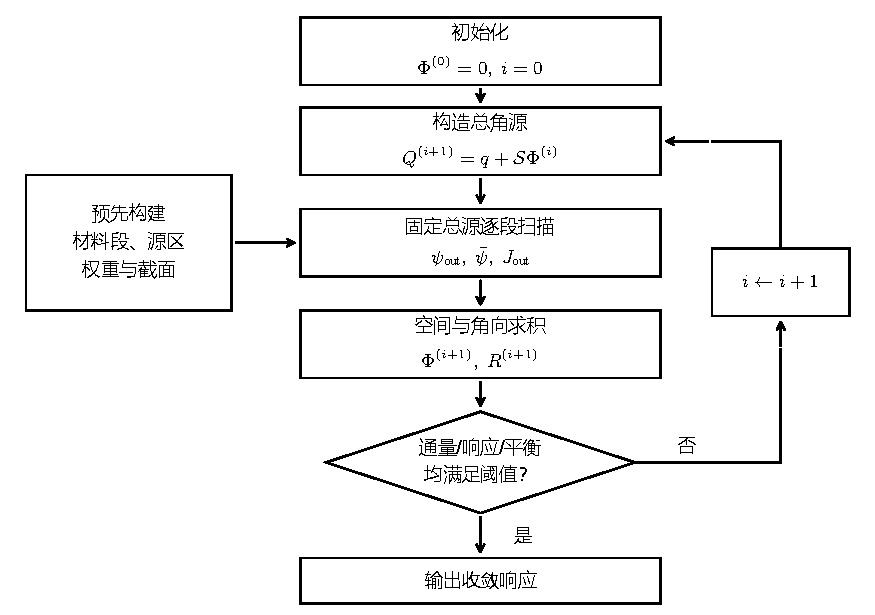
\includegraphics[width=0.95\linewidth]{figures/v21_moc}
\caption{多群固定源MOC的源迭代}\label{fig:moc}
\end{figure}

CMFD通过求解粗网中子平衡方程，减小源迭代中衰减较慢的误差分量，其粗网界面中子流由MOC扫描结果计算\upcite{5}。Random Ray随机采样射线的位置和方向，沿射线求解输运方程并累加源区通量\upcite{21}。已有MOC实现多利用栅元重复或堆芯结构。在非重复几何中，不同轨迹的长度和材料段数不同。

\subsection{MOC 数值误差与空间精度控制方法}
几何误差以体素几何与参考几何中的材料边界、材料次序和段长差异评价。保持其余参数不变，分别改变轨迹间距、源区尺寸与源项阶次、离散方向数与散射展开阶次，考察相应响应的收敛。迭代误差则通过收紧收敛阈值检查。

均匀细化便于检查解随网格加密的收敛情况，但也会加密对指定响应影响很小的区域。按材料界面细化用于减小界面位置和材料段长的偏差，按通量梯度细化则依据局部通量的空间变化确定细化位置。目标导向方法结合正向解与伴随解，估计各处离散误差对指定响应的贡献，据此确定需要细化的区域。Liu等用多层非匹配笛卡尔网格表示局部细化后不同尺寸的单元\upcite{16}。Wang与Ragusa在采用$S_N$离散的非结构网格上比较常规自适应细化与目标导向细化，Lathouwers在目标误差估计中保留完整的角向依赖，Baker等用子网格校正构造固定源输运残差\upcite{22,23,24}。Goffin等以有效增殖因子为目标量估计误差，并据此调整非结构网格单元在不同空间方向上的尺寸\upcite{25}。

Liu等在三维$S_N$中结合空间矩比指标、多层数据结构与扫描优化，对所测强非均匀问题，相同精度下较均匀细化节省60\%—80\%计算成本\upcite{26}。Liu等的后续研究采用通量重构和对偶加权残差（DWR），在所测多群固定源与临界问题的相近目标精度下减少超过70\%的工作量和运行时间\upcite{27}。Balakovo-3固定源剂量基准中，多层八叉树将约950万单元减至190万，对常规$S_N$计算及实验的均方根差异分别约4\%与10\%，相对均匀细网格节省约70\%成本\upcite{28}。Wilson等进一步将等几何离散的目标误差、局部$h(p)$细化和扩散加速结合\upcite{29}。

上述目标导向研究结合数值解的空间重构与伴随解，估计局部离散误差对指定响应的影响，据此选择细化区域，减少不必要的全域加密。体素化MOC需要分别考察几何映射与输运离散的影响。评价几何误差时，比较同一射线在参考几何与体素几何中的材料次序和段长，分析这些差异对碰撞损失与散射源积分的影响。检查输运离散误差时，固定材料分布，分别减小轨迹间距、细分源区及增加离散方向，比较指定响应的变化。结合伴随解，可估计各区域误差对响应的影响，并选择细化位置。细化增加的材料段数和源区数量可用于估计新增计算量，再结合实际耗时，比较细化前后的响应误差与计算代价。



\section{GPU-MOC并行算法研究现状}\label{sec:3}

\subsection{三维MOC计算流程与并行特征}

几何与材料确定后，构建轨迹并确定材料段，给定本轮总源与入射边界角通量后沿轨迹扫描。每条轨迹按材料段顺序计算，前一段的出射角通量作为后一段的入射角通量。不同完整轨迹可以并行执行，各轨迹对同一源区的段积分完成求和后，才能构造下一轮源项。当所有能群的散射源均由上一轮通量计算时，各能群可同时扫描，这对应群Jacobi迭代。若计算完一个能群就用其新通量更新其他能群的散射源，则依赖该结果的能群须在更新后扫描。

真空外边界的入射角通量为零，一条完整轨迹的入口值不需要由另一条轨迹提供。反射或周期边界则按边界对应关系，将出射角通量作为另一条轨迹的入射值。采用迭代更新边界角通量时，各轨迹使用上一轮的边界值扫描，轮末再更新下一轮的入射值。图\ref{fig:3}给出轨迹、材料段计算及源区通量求和之间的关系。

\par\medskip\noindent\begin{minipage}{\linewidth}
\centering
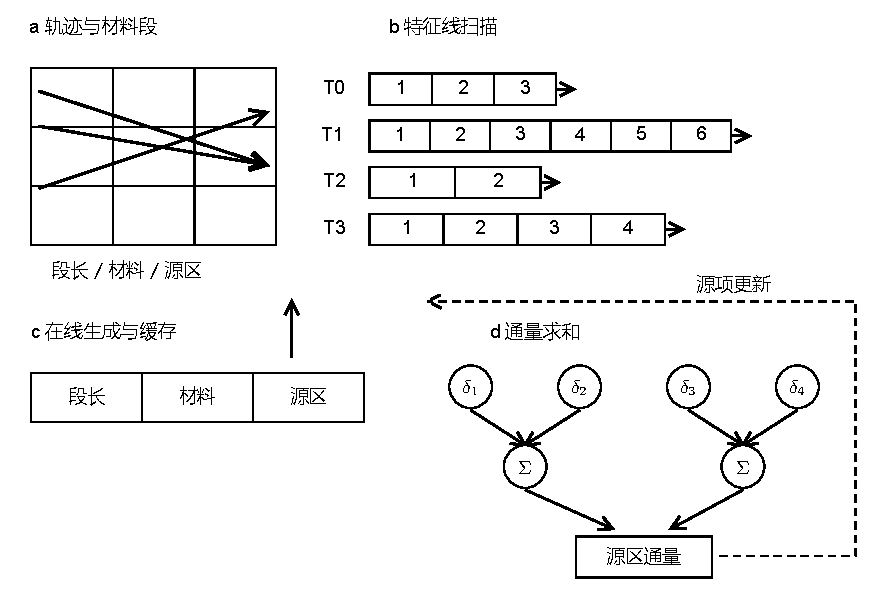
\includegraphics[width=0.95\linewidth]{figures/fig3}
\captionof{figure}{GPU-MOC轨迹扫描与通量求和\upcite{30,31,7,32,8,33,34}。 (a) 轨迹与材料段。(b) 线程沿特征线逐段计算角通量。(c) 在线生成与缓存。(d) 通量求和。}
\label{fig:3}
\end{minipage}\par\medskip

\subsection{CPU-GPU异构并行与任务划分}

CPU与GPU协同完成几何处理、轨迹准备、扫描、通量求和及源更新。GPU扫描所需的材料截面、源项和材料段，先从CPU内存传入GPU显存。截面按材料和能群存放，源项按源区和能群存放，扫描根据各段的材料编号和源区编号读取相应数据。若源更新也在GPU上完成，通量和源项数组可在迭代期间保存在显存中，CPU接收所需区域通量、反应率，以及相邻两轮的通量与反应率变化量和中子平衡偏差，用于输出结果和判断收敛。

STREAM3D-GPU逐个轴向平面执行输运计算\upcite{33}。计算某一平面前，将其入射角通量传入GPU显存，计算后向CPU内存返回出射角通量，以及用于粗网加速的界面中子流，截面等固定数据继续保存在显存中\upcite{35}。沿给定轴向传播方向，后一平面的入射数据由前一平面的出射结果提供，须在这些数据准备好后扫描。其会议算例采用七群、64个轴向平面的C5G7，两颗EPYC 7543共64核的CPU计算与同一主机加8块RTX A5000相比，MOC求解器耗时由1368 s降至34 s，程序总耗时由1704 s降至100 s\upcite{35}。表\ref{tab:2}另列2026年四分之一堆芯算例的显存与求解结果。

宋佩涛等使CPU与GPU的计算任务、数据传输和输运扫描在时间上部分重叠\upcite{32,36}。例如，GPU扫描当前轨迹批时，可将下一批所需段数据传入另一缓冲区，减少GPU等待数据传输完成的时间。两个缓冲区同时占用内存或显存，各批对源区通量的贡献全部求和后，再更新源项。局部细化后，需要重新准备的数据量取决于穿过修改区域的轨迹。

\subsection{特征线存储与GPU显存管理}

每个材料段记录段长、材料编号和源区编号，轨迹方向与入口角通量按轨迹保存。计算还需按源区和能群保存标量通量，以及构造各向异性散射源所需的通量角矩。采用线性源时，另存源项的空间变化系数。

材料段可以在轨迹构建后全部保存，以后各轮扫描读取同一套段长和编号。也可以在扫描过程中在线生成，每轮扫描重新追踪，以减少需要保存的材料段数据。部分缓存则只保存一部分轨迹，其余轨迹在线生成。Zhou等优先保存段数较多的轨迹，并把二维轨迹、极角和轴向位置的组合分配给GPU线程\upcite{30}。段数据不能全部保存在显存时，可将预存轨迹分批送入设备，完成扫描后替换为下一批。预存与在线生成的区别在于读取已有材料段，还是在扫描时重新追踪。轨迹分批处理控制同时保存在显存中的数据量。

几何、轨迹和源区划分固定时，预存的段长、材料编号和源区编号可在后续源迭代中重复使用。对于包含重复栅元的几何，模块化追踪可共用重复栅元内的局部轨迹段数据\upcite{18}。

对于各轴向层共用同一二维径向网格的几何，Song等只保存二维径向材料段，扫描时根据射线与轴向分层平面的交点生成三维材料段\upcite{7}。相对于平源、显式保存全部三维材料段的基线，该方法同时采用线性源和轨迹分批处理。线性源用一次函数表示源区内的源项，在相应精度要求下减少源区与分段数。轨迹分批处理只将当前批的轨迹数据和边界角通量保存在显存中，其余批次依次送入。非重复体素几何局部细化后，则需检查哪些缓存轨迹穿过了被修改的单元，并更新这些轨迹的分段。

NuDEAL在各轴向层共用二维径向网格的三维C5G7 DGMOC算例上，改变每一批包含的角度数\upcite{34}。每批角度由2增至32时，显存明显增加，单次输运扫描的时间变化很小。该算例中每个角度已经包含大量单元上的计算。增加同批角度，主要增加同时留在显存中的角通量和相关数组。一批放入多少角度，由剩余显存和每个角度已有的任务量共同决定。图\ref{fig:4}给出该算例的显存与时间。

\par\medskip\noindent\begin{minipage}{\linewidth}
\centering
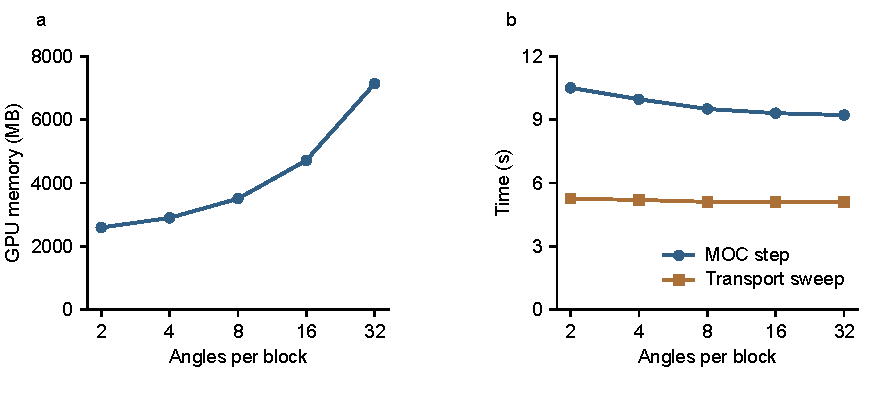
\includegraphics[width=0.95\linewidth]{figures/fig4_nudeal}
\captionof{figure}{NuDEAL三维C5G7 DGMOC的显存与时间\upcite{34}。 (a) GPU显存随每批角度数的变化。(b) 同一算例的MOC耗时（原文Single MOC time）和单次输运扫描耗时。}
\label{fig:4}
\end{minipage}\par\medskip

\subsection{GPU任务调度与负载均衡}

局部细化、薄层和孔道会使各轨迹的材料段数和层级访问次数不同。一个线程负责一条轨迹时，同一线程束中段数较少的线程先完成计算，线程束仍需继续执行其余轨迹段。按段数分组可以减少这种等待，按空间位置分组则使相邻线程读取相近的材料和源区。

二维OpenMOC在GPU上将一条轨迹的一个能群分配给一个CUDA线程，由该线程沿轨迹逐段计算角通量并累加源区通量。其CPU向量化求解器将能群循环置于内层，并沿能群维度进行SIMD向量化\upcite{5}。方位角数量从4增加到128时，可分配给GPU线程的轨迹—能群组合数量随之增加。Wang等在CPU上把轴向分层几何的循环轨迹分成更细的任务，并按估计计算量分配处理器\upcite{37,38}。ANT-MOC在同一次全堆芯计算中同时计入存储、计算和通信，并在节点、GPU和计算单元上分配任务\upcite{8}。

许多轨迹将加权段积分累加到式\eqref{eq:tally}的同一源区。若干线程同时向该源区累加时，原子加使每一次相加都完整写入，已得到的结果不会被另一次写入覆盖。先在线程块内合并写入同一源区的贡献，再通过原子加累加到全局通量数组，减少全局原子加的次数。局部求和需要共享内存，并在线程块内同步\upcite{31,39}。

几何与源区划分固定时，按段数或空间位置建立的分组可用于后续源迭代。局部细化改变部分轨迹的段数与源区访问，调度需要更新这些任务的工作量估计。比较调度方式时，分组和求和的额外处理与扫描耗时共同构成迭代成本。


\begin{longtable}{@{}>{\raggedright\arraybackslash}p{\dimexpr0.18\linewidth-1.5\tabcolsep\relax}>{\raggedright\arraybackslash}p{\dimexpr0.22\linewidth-1.5\tabcolsep\relax}>{\raggedright\arraybackslash}p{\dimexpr0.24\linewidth-1.5\tabcolsep\relax}>{\raggedright\arraybackslash}p{\dimexpr0.36\linewidth-1.5\tabcolsep\relax}@{}}
\caption{代表性MOC并行方法的结构条件与计算结果}\label{tab:2}\\
\toprule
研究与几何 & 所用办法 & 依赖的结构条件 & 代表结果 \\
\midrule
\endfirsthead
\toprule
研究与几何 & 所用办法 & 依赖的结构条件 & 代表结果 \\
\midrule
\endhead
\bottomrule
\endlastfoot
OpenMOC\upcite{5}，二维C5G7七群 & GPU按轨迹和能群分配线程，CPU对能群内循环向量化 & 给定源项后，不同轨迹与能群的扫描可分别计算 & 四种NVIDIA GPU，相对单颗Xeon核的本征值求解最大加速近50倍 \\
Song等\upcite{7}，少群三维组件及SMR & 线性源、在线轴向追踪、轨迹分批处理 & 轴向分层。基线为平源和显式三维分段 & 25 cm组件基线22129 MB。三项合用后组件显存降低98.5\%，单GPU可计算四群SMR全堆芯本征值 \\
Wang等\upcite{37}，轴向分层CPU-MOC & 循环轨迹细分，按估计计算量分配 & 轴向分层几何中的循环轨迹 & 10240至98304个CPU核，并行效率大于40\% \\
ANT-MOC\upcite{8}，三维全堆芯 & 存储、计算与通信代价，三级任务分配 & 全堆芯轨迹同时受容量和设备间负载约束 & 约$10^{11}$条轨迹，16000 GPU。强扩展效率70.69\%，弱扩展效率89.38\% \\
STREAM3D-GPU\upcite{33}，OPR四分之一堆芯 & 逐轴向平面处理，异步执行 & 轴向分解的MOC/DD，平面之间传递角通量 & 每个MPI进程所需的GPU显存由约50 GB降至4.5 GB以下。8 GPU与16 GPU相对128核CPU的本征值求解加速分别为22.1倍和40.5倍 \\
NuDEAL\upcite{34}，轴向分层几何DGMOC & 按方位角分批，逐平面计算轴向矩 & 轴向分层。单个角度内已有大量单元任务 & RTX 2080 Ti上的三维C5G7。每批角度由2增至32时，显存由2589 MB增至7133 MB，扫描时间由5.25 s变为5.09 s。64个角度同时驻留时超出显存 \\
\end{longtable}

已有GPU-MOC方法利用轴向分层、重复栅元或全堆芯分解，协调轨迹保存、扫描和通量求和。复杂体素几何的局部细化则使轨迹段数、访问单元和缓存有效性同时变化。可据局部网格与轨迹的穿越关系识别更新范围，再以轨迹生成成本、读取量和预计复用次数选择缓存与任务分组。


\section{聚变屏蔽应用与数值验证依据}\label{sec:4}
验证对象包括厚屏蔽体、多材料分层、薄层与斜交界面，以及直孔道和折弯孔道。厚屏蔽体中主要比较通量和反应率随穿透深度的变化，多材料分层中比较中子经过不同材料后的能谱和反应率。薄层与斜交界面用于检查体素划分对材料段长的影响，孔道计算检查体素几何是否保留孔道连通性，并比较轨迹间距和离散方向变化对孔道出口响应的影响。

\subsection{聚变屏蔽基准与实验验证依据}\label{sec:benchmark}
Kobayashi三维基准采用嵌套空腔、直孔道和折弯孔道三种几何，图\ref{fig:benchmark_geometries}(a)给出折弯孔道的材料区域。源区与屏蔽区总宏观截面为$0.1\ \mathrm{cm}^{-1}$，近真空区为$10^{-4}\ \mathrm{cm}^{-1}$，均匀各向同性体源强度为$1\ \mathrm{n\,cm}^{-3}\mathrm{s}^{-1}$。每种几何分别设置纯吸收和散射比$\Sigma_s/\Sigma_t=0.5$两种情况，共六个单群问题。该基准以三个坐标平面为反射对称面。纯吸收问题采用输运积分计算得到的通量作为参考，含散射问题采用GMVP蒙特卡罗计算结果作为参考\upcite{40,41}。本计划采用LANL报告附录的全空间展开输入、真空外边界和相应源归一化，并核对其MCNP点通量结果\upcite{42}。该基准采用预设宏观截面。沿指定射线核对材料次序和段长，改变轨迹间距、离散方向数和迭代阈值，比较参考点通量的变化。

FNG-ITER流束实验由不锈钢、有机玻璃和前端铜层组成，屏蔽体正面为$100\times100\ \mathrm{cm}^2$、厚94.26 cm，内部直孔道长39.07 cm、内径2.8 cm，末端连接测量空腔\upcite{43}。图\ref{fig:benchmark_geometries}(b)展示分层材料、直孔道和空腔的关系。轴上工况的源与孔道对齐，距屏蔽体前表面5.3 cm，偏轴工况将源横向移动5.3 cm。采用轴线上13个位置的$^{93}$Nb$(n,2n){}^{92m}$Nb、$^{27}$Al$(n,\alpha){}^{24}$Na和$^{58}$Ni$(n,p){}^{58}$Co反应率，空腔内11个位置的前两种反应率，以及偏轴照射下15个位置的$^{93}$Nb$(n,2n){}^{92m}$Nb反应率，共六组曲线、76个测量值及其误差\upcite{44,45}。比较轴上与偏轴照射时孔道、空腔及屏蔽体后方的反应率分布，检查程序对源位置变化和孔道流束的计算。

\par\medskip\noindent\begin{minipage}{\linewidth}
\centering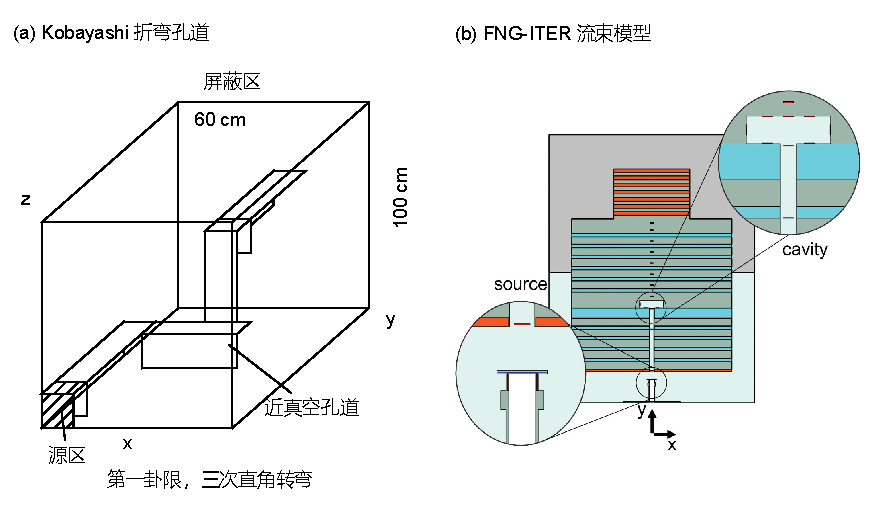
\includegraphics[width=0.95\linewidth]{figures/benchmark_geometries}
\captionof{figure}{三维中子屏蔽与孔道流束基准的几何结构。(a)Kobayashi折弯孔道基准的材料区域\upcite{40}。(b)FNG-ITER流束实验的屏蔽结构与测量布置\upcite{45}。}\label{fig:benchmark_geometries}
\end{minipage}\par\medskip

FNG钨实验将厚49 cm的钨合金屏蔽体置于14 MeV D-T源前，源距前表面5.3 cm，图\ref{fig:benchmark_responses}(a)示意中央测量层及活化箔位置\upcite{46,47}。选取$^{93}$Nb$(n,2n){}^{92m}$Nb、$^{90}$Zr$(n,2n){}^{89}$Zr、$^{27}$Al$(n,\alpha){}^{24}$Na、$^{56}$Fe$(n,p){}^{56}$Mn、$^{58}$Ni$(n,p){}^{58}$Co、$^{197}$Au$(n,\gamma){}^{198}$Au和$^{55}$Mn$(n,\gamma){}^{56}$Mn七种反应。四个测量层内，各反应箔的中心深度略有差别，分别位于4.94—5.10、14.94—15.10、24.94—25.10及34.94—35.10 cm范围内，每种反应各有4个测量值，共28个，所选数据均附实验误差\upcite{44}。不同反应对中子能区的响应不同，其随深度的变化用于检验厚钨屏蔽中的中子衰减和散射慢化，计分采用各箔的实际位置、体积和反应定义。

OKTAVIAN铜球实验在球心设置D-T源，铜材料外半径30 cm，不锈钢球壳厚0.5 cm，并保留束流管孔。实验以飞行时间法测量泄漏中子谱，公开基准数据集收录了140个能区的实验谱值及其误差，能量范围为0.076399—20.66 MeV\upcite{44}。van der Marck给出了MCNP计算与实验的谱比较\upcite{48,49}，图\ref{fig:benchmark_responses}(b)采用其中MCNP-4C3与JEFF-3.1的同组能谱和C/E结果。比较各测量能区的泄漏中子谱及C/E随能量的变化，检查球面几何中的中子输运与泄漏能谱计算。上述三组实验采用OpenMC Fusion Benchmarks公开模型中的材料、源分布和测量位置，分别按活化反应率和球壳外表面泄漏中子流的计分定义计算\upcite{44}。

\par\medskip\noindent\begin{minipage}{\linewidth}
\centering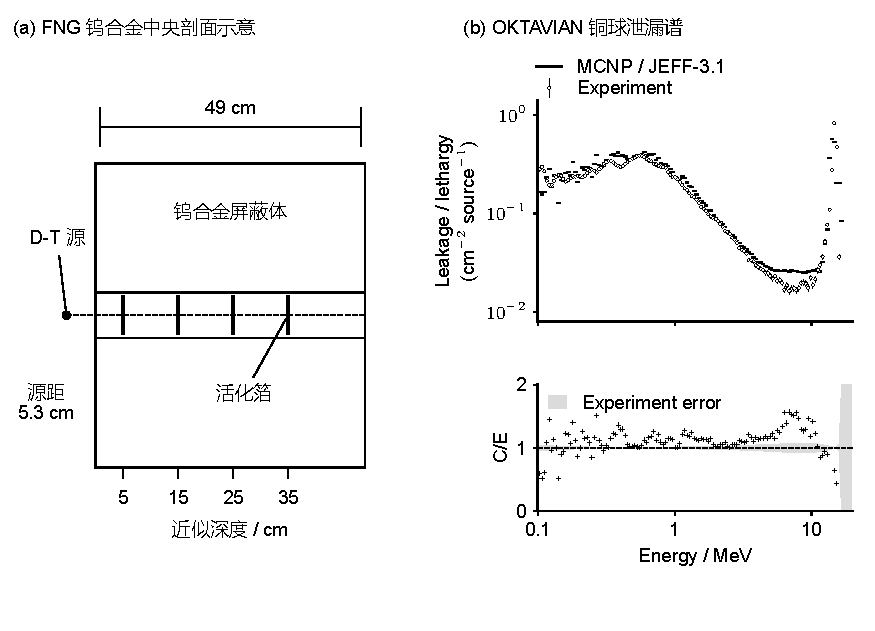
\includegraphics[width=0.95\linewidth]{figures/benchmark_responses}
\captionof{figure}{聚变中子屏蔽实验布置与代表性响应。(a)FNG钨合金屏蔽体中央剖面与活化箔位置\upcite{44,47}。(b)OKTAVIAN铜球泄漏中子谱的MCNP-4C3/JEFF-3.1计算与实验比较\upcite{48}。上图为每源中子、单位面积及单位对数能量宽度的泄漏中子流谱，下图为计算值与实验值之比C/E。}\label{fig:benchmark_responses}
\end{minipage}\par\medskip

\subsection{数值正确性与独立程序比较}\label{sec:verification}
数值正确性的依据包括纯吸收问题的解析解、参考几何中的材料交点，以及Kobayashi基准的参考点通量。将追踪得到的材料次序和段长与参考几何求交结果比较。将出射角通量和段平均角通量与解析解比较，再检查轨迹求积得到的区域体积及全域中子平衡。分别减小体素尺寸和轨迹间距，提高源项近似阶次及增加离散方向，检查指定响应的变化。CPU与GPU采用相同的材料段、源区、求积权重和收敛阈值，逐项比较出射角通量、源区通量及最终响应。

独立计算采用OpenMC的多群与连续能量模式\upcite{50}，并选用具有公开网格、截面与固定源接口的OpenSn作为$S_N$对照\upcite{51}。在相同体素几何和多群数据下比较独立程序的结果，检查输运离散的影响。比较参考几何与体素几何的计算结果，分析材料映射的影响。比较多群与连续能量计算结果，分析能群处理的影响。各项比较保持其他物理输入量相同。多群程序比较采用相同的群常数和散射展开阶次，角向求积采用相同的权重归一化约定。多群与连续能量比较采用相同的评价核数据来源、几何和源设置。所有比较均统一源强、计分定义及归一化。具体对照顺序见第5.5节。

实验比较采用\ref{sec:benchmark}节的测量位置、反应和能区，列出C/E、实验误差与蒙特卡罗统计误差。保持几何和源设置相同，替换评价核数据库，比较核数据选用造成的结果差异。

\subsection{GPU 异构并行性能与完整计算效率评价}\label{sec:performance}
GPU性能评价以经过数值检查的CPU并行实现为基线，保持几何、材料段、源区、能群、离散方向、数值精度与收敛阈值相同。扫描加速比与整体加速比分别采用CPU和GPU的扫描耗时之比、完整求解耗时之比。完整求解耗时按程序开始读取几何和核数据至全部计算完成并输出收敛响应之间的实际经过时间计算，包含轨迹准备、设备初始化、传输、扫描、通量求和及源更新。结束计时前，同步尚未完成的GPU任务\upcite{39}。传输与计算重叠时，重叠区间在总耗时中只计一次。

分别记录材料段生成或读取、特征线扫描、通量求和、CPU与GPU间数据传输及同步等待的耗时，比较各阶段对总耗时的贡献。记录求解过程中GPU显存占用的最大值，并区分材料截面、源项与通量数组、材料段缓存、批次输入输出缓冲区及临时计算数组的占用。在相同离散条件下比较CPU与GPU的求解时间。在满足相同响应误差容限的条件下，比较不同网格和执行参数所需的完整计算时间及峰值显存。

\subsection{聚变屏蔽应用与混合计算评价}\label{sec:hybrid}
CADIS以给定区域内的反应率为目标量构造伴随源，求解伴随通量，再据此生成随位置和能量变化的权窗及源偏倚分布\upcite{52}。反应率对应的伴随源由计分区内的分群宏观反应截面及计分归一化确定，区外取零。源抽样采用偏倚分布，粒子初始权重按原始源与偏倚源的概率比设置，输运中通过分裂与轮盘赌控制权重。

FW-CADIS先求正向通量，估计多个计分量，再以各响应估计的倒数加权对应伴随源，使所关注位置或能区的相对统计误差更加均匀\upcite{53}。MOC在体素几何上计算正向与伴随通量，并生成蒙特卡罗计算所需的减方差参数。蒙特卡罗粒子在未经体素化的基准几何模型中追踪。

以厚屏蔽深部及孔道外各测点的反应率，比较MOC辅助减方差前后的蒙特卡罗计算效率。混合计算总时间包括MOC求解、减方差参数生成与转换、蒙特卡罗输运，以及选择减方差参数所需的试算。逐个测量位置列出反应率估计值及其相对统计误差，比较相同总时间下的统计误差，以及全部关注测点达到预设相对统计误差上限所需的总时间。

\section{研究内容、技术路线与实施方案}\label{sec:5}
\subsection{总体研究思路与技术路线}
申请人将参与体素化MOC程序开发，围绕三维、多群、稳态固定源中子输运，开展材料路径误差控制、GPU异构并行及精度与成本协同选择三项研究。几何以规则体素为基础，通过局部层级细化表示材料界面、薄层和孔道。采用第二章的角通量计算、源区求积和多群源迭代建立CPU数值基线，再扩展伴随求解、局部细化与GPU执行。

程序开发参考OpenMOC公开的平源扫描与源迭代实现\upcite{5}，将几何追踪、段数据、源区积分和计算执行接口分开。先实现二维规则体素的材料分段和固定源求解，再扩展三维网格穿越、各向异性转移及层级单元。各模块采用解析算例，与按第二章离散公式建立的CPU参考实现逐项对照。

图\ref{fig:research_plan}给出计算与方法研究的关系。几何输入和材料映射产生体素材料场，特征线生成与分段为多群扫描提供有序材料段，源区求和与源更新得到通量和指定响应。误差控制研究给出细化位置及离散参数，GPU异构并行研究处理相应的轨迹更新、缓存和扫描任务，两者产生的误差指标与计算工作量共同用于选择离散和执行配置。选定配置用独立算例比较响应误差、求解时间及峰值显存。

\par\medskip\noindent\begin{minipage}{\linewidth}
\centering
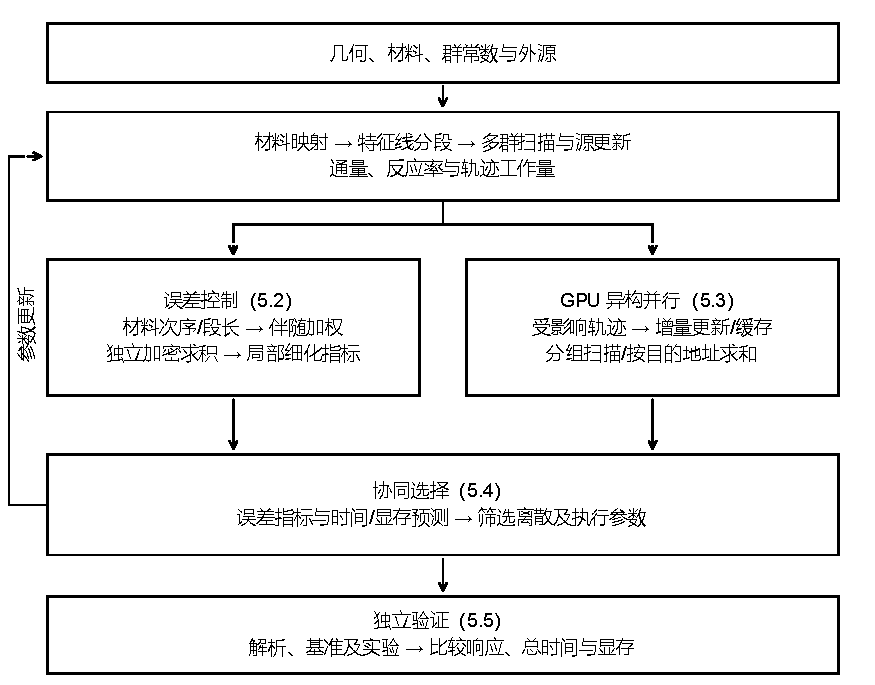
\includegraphics[width=0.95\linewidth]{figures/research_plan_v21}
\captionof{figure}{体素化MOC误差控制与GPU异构并行研究路线}
\label{fig:research_plan}
\end{minipage}\par\medskip

\subsection{复杂几何体素化 MOC 特征线追踪与误差控制}
材料体积接近并不意味着射线经过各材料的次序和长度接近。以原CAD/CSG或解析几何作为参考，对同一射线分别生成参考材料段和体素材料段，按两组界面的全部交点划分共同区间。在这些区间上比较材料编号、总截面及转移截面，计算各材料的路径长度与分群光学厚度。

从固定源问题$\mathcal L\psi=q$与响应$R=\langle d,\psi\rangle$出发，采用伴随方程$\mathcal L^\dagger\psi^\dagger=d$评价材料表示改变的影响。以体素模型为展开点，将参考模型与体素模型之差记为$\delta$，一阶响应变化为
\begin{equation}
\delta R\approx\langle\delta d,\psi\rangle+
\langle\psi^\dagger,\delta q-\delta\mathcal L\psi\rangle.
\label{eq:response_perturbation}
\end{equation}
$\psi$和$\psi^\dagger$分别为正向与伴随角通量，$q$为外源，$d$为计分响应函数。内积对空间和方向积分并对能群求和，外边界及边界条件保持相同。离散伴随按正向离散及求积权重的加权转置构造，以$\langle d,\psi\rangle=\langle\psi^\dagger,q\rangle$检查响应互易关系。$\delta q$表示源分布变化，$\delta d$表示计分区域或响应函数的表示变化。材料变化在输运算子中的作用写为
\begin{equation}
(\delta\mathcal L\psi)_g(\mathbf r,\Omega)
=\delta\Sigma_{t,g}\psi_g(\mathbf r,\Omega)
-\sum_{g'}\int_{4\pi}\delta K_{g'\to g}(\mathbf r,\Omega'\to\Omega)
\psi_{g'}(\mathbf r,\Omega')\,d\Omega'.
\label{eq:material_operator_perturbation}
\end{equation}
几何界面移动改变射线在哪些区间使用某种材料，因而改变总碰撞损失和转移源。按式\eqref{eq:response_perturbation}，在各共同区间上计算外源和材料变化的伴随加权贡献，再计入相应单元，连同响应函数变化项得到局部响应估计。保留各项的正负号，比较相同段长偏差在不同位置和能区引起的响应增减。通过小幅移动界面、改变薄层厚度和孔径，比较估计值与重新求解所得的实际响应变化，检验一阶近似的适用尺度。

几何影响与MOC离散影响分别计算。前者在相同轨迹、角向求积和源项近似下改变材料表示，后者固定体素材料分布，在加密轨迹、细分源区或增加离散方向后检查粗解。借鉴已有伴随误差估计和通量重构方法\upcite{24,27}，将粗角通量重构到独立加密的离散空间，构造
\begin{equation}
\rho_F=q_F-\mathcal L_F P_F\psi_h,
\qquad
\eta^{\rm num}_j=\langle\psi_F^\dagger,\rho_F\rangle_j.
\label{eq:independent_residual}
\end{equation}
$F$为固定材料分布的加密离散，$j$为局部单元或网格块。重构$P_F$以材料区、源区和计分区的交叠区域为单位，将粗解的平均角通量赋给加密子单元，保持该区域细化前后的体积加权平均值。增加离散方向时，以粗解的通量角矩约束新方向的角通量，并核对标量通量和反应率积分。$\rho_F$为加密空间中的残差，$\psi_F^\dagger$为相应伴随近似。指标评价时间包括重构、补充扫描和伴随求解。分别改变轨迹间距、源区尺寸、源项阶次和离散方向，检查各项估计与响应收敛的对应关系。

局部细化先保留几何特征，再根据响应影响分配分辨率。对穿过薄层两侧界面的单元检查材料交点，对孔道检查原几何与体素模型中的连通关系，优先细化未保留这些特征的单元。其余单元以几何扰动和输运离散的局部响应估计排序，试分割候选单元，统计新增材料段、源区和追踪查询次数，结合预计响应误差下降选择细化单元，再更新网格并进行全局源迭代。

对均匀细化、材料界面细化、通量梯度细化和上述响应驱动细化使用相同外源、核数据与迭代判据。解析几何、斜交界面、薄层及直通和折弯孔道分别改变界面位置、倾角和特征尺寸，比较材料段、反应率与独立高精度参考结果的偏差、估计值与该偏差之比，以及完整计算成本，分别检验几何保护和伴随加权对细化结果的影响。

\subsection{面向复杂体素几何的CPU-GPU协同并行}
GPU异构并行以经验证的CPU求解器为参照，先采用CPU准备几何与轨迹、GPU完成扫描和源区求和的计算方式，再比较GPU在线追踪与扫描相连的方式。CPU负责层级网格修改、细化选择和轨迹状态管理，GPU读取材料与源项计算角通量、通量矩和响应。源更新逐步移至GPU端，截面等固定数据保存在显存中，通量和源项在GPU端逐轮更新。任务划分的研究对象是几何处理与扫描之间的工作量变化，以及准备、传输和同步在完整求解中的代价。

局部细化后的轨迹更新采用“网格块—轨迹”反向索引。建立轨迹时记录其穿过的网格块及区间，网格块改变后据此取得候选轨迹，只对这些轨迹与修改块相交的区间重新分段，并与未改变的前后段序列连接。单元采用稳定的层级编号，通过映射表访问当前源区数组，避免局部细化因整体重新编号而使全部段记录失效。轨迹缓存记录所依赖网格块的几何与源区划分版本，读取前按版本判断有效性。轨迹位置、方向集合或求积规则改变时重新建立相应轨迹与索引。更新后的材料段与全量重建逐段对照，并对新离散模型重新进行全局源迭代。

缓存选择同时考虑生成成本、读取成本和复用次数。在显式存储、在线生成和部分缓存三种方式之间比较，部分缓存为每条轨迹或轨迹批估计后续扫描次数，以及在线生成与缓存读取的时间差，扣除缓存维护、加载和失效重建的成本。以预计节省时间与缓存字节数之比选择需要保存的轨迹批，显存同时为源项、通量矩和批次工作数组留出空间。预计复用次数以当前网格版本剩余的扫描为限，根据源迭代剩余轮数及每轮任务安排估计，网格或源区划分改变后重新评价失效的缓存。局部细化频率及其引起的失效范围作为缓存策略的输入，比较长轨迹优先与成本估计驱动两种选择。

扫描任务从轨迹与能群的组合出发，保持同一轨迹的角通量逐段依赖。依据段数和层级访问次数估计任务工作量，比较轨迹生成顺序、按段数分组、按空间位置分组，以及先按空间块再按段数分组的方式。源区通量计算比较直接原子加与线程块内局部求和（并行归约）。局部求和按源区、能群及通量矩编号合并写入同一地址的段积分，再以原子加累加到全局数组。没有可合并贡献时，仍以原子加写回。分组更新、共享内存占用和求和同步均计入成本。

固定材料和层级索引保存在GPU显存中，轨迹批与所需角通量缓冲在CPU内存和GPU显存之间传输。两个缓冲轮换时，CPU准备或传输下一批，GPU扫描当前批，源区通量完整汇集后再更新源项。比较串行准备与扫描、异步传输重叠，以及GPU在线生成的实际时间线，记录CPU处理、链路传输、GPU计算和同步。通过全量与增量更新、三种存储、按生成顺序与分组调度、直接原子加与局部求和、不同异构任务划分的对照，分析轨迹变化比例、工作量差异及缓存复用对完整求解效率的影响。

\subsection{体素离散与GPU执行的精度–成本协同优化}
体素细化既改变材料表示，也改变材料段数、源区数和GPU访问的数据。第二项研究得到的最优执行配置因而随离散变化，第一项研究选择的细化位置也对应不同的追踪与求和代价。以响应误差、完整时间和峰值显存为共同评价量，研究有限试算条件下的离散与执行参数选择。

令$\theta$表示体素尺寸、局部细化层级、轨迹间距、源区划分、源项阶次和离散方向，$s$表示缓存选择、轨迹批量、任务分组、通量求和方式及CPU与GPU任务划分。在固定物理模型和能群数据下，选择问题写为
\begin{equation}
\begin{aligned}
\min_{\theta,s}\quad &T_{\mathrm{total}}(\theta,s),\\
\text{s.t.}\quad &\widehat e_{\mathrm{resp}}(\theta)\leq\varepsilon_{\mathrm{resp}},\\
&\Delta_{\mathrm{impl}}(\theta,s)\leq\varepsilon_{\mathrm{impl}},\\
&\widehat M_{\mathrm{peak}}(\theta,s)\leq M_{\mathrm{avail}}.
\end{aligned}
\label{eq:joint_selection}
\end{equation}
第$d$个响应的几何局部估计记为$\eta^{\rm geo}_{j,d}$，由式\eqref{eq:response_perturbation}的局部贡献得到，输运离散估计$\eta^{\rm num}_{j,d}$由式\eqref{eq:independent_residual}得到。选参指标采用局部估计绝对值之和：
\begin{equation}
\widehat e_{\mathrm{resp}}=
\max_d\frac{c_d\sum_j\bigl(|\eta^{\rm geo}_{j,d}|+|\eta^{\rm num}_{j,d}|\bigr)}{a_d+|R_d|}.
\label{eq:response_indicator}
\end{equation}
$c_d\geq1$为校准系数，根据校准算例中参考响应偏差与局部绝对值之和的比值确定，并在独立几何上检验。$a_d$沿用式\eqref{eq:convergence}的绝对尺度。$\Delta_{\mathrm{impl}}$是在相同离散输入下CPU与GPU的通量及响应差异，按式\eqref{eq:convergence}的尺度归一化并以CPU结果作为比较基准，$\widehat M_{\mathrm{peak}}$为预测峰值显存，$M_{\mathrm{avail}}$为可用显存。其中$\varepsilon_{\mathrm{resp}}$是响应精度要求，与式\eqref{eq:convergence}的迭代变化阈值$\varepsilon_R$分别设置。迭代阈值取到足以分辨所考察离散误差的水平。实现差异先用代表性轨迹、源区和完整算例验证各执行配置，再对选定配置进行复核。

误差指标以已知参考结果的几何进行校准，比较估计值与参考响应偏差随细化的变化，确定式\eqref{eq:response_indicator}的校准系数。实际选择使用可计算指标，独立高精度结果用于事后验证。参考解的不确定度由解析精度、参考离散收敛或蒙卡统计误差给出，与CPU-GPU实现差异分别报告。几何尺寸、倾角和孔道结构按算例划分建模与独立验证集合，同一几何的不同网格不跨集合充当独立测试。

成本预测使用完整求解前可取得的单元与源区数量、抽样射线段数、层级访问次数、同一线程束内的重复读取比例和同址写入比例、缓存字节数、任务工作量分布，以及GPU计算、访存和CPU—GPU链路特征。在同一扫描步抽样截面与源项读取地址、通量写入地址，以活跃线程数为分母，分别统计参与重复读取和同址写入的线程比例。用少量准备与扫描试算标定材料段生成、缓存读取、求和及传输模型，按任务依赖的关键路径估计重叠后的耗时。源迭代次数先由相近问题估计，形成稳定下降后，用通量变化、响应变化和中子平衡偏差的连续迭代比值估计下降率，预测达到各阈值所需的剩余轮数，取最大值并逐轮更新。预测峰值显存按同时存活的数组和批次缓冲计算，并与实测峰值比较。目标总时间包括模型标定、候选搜索（含误差评价与试算）、选定配置的完整求解及复核。完整求解按第4.3节计时，包含轨迹准备与更新。单次求解承担本次建模与搜索支出，重复设计计算则同时报告累计时间与模型复用次数。

根据可选网格层级和GPU配置生成候选方案，筛除未保留指定几何特征的方案，再用误差与显存预测筛选，以时间预测选择试算对象，并用实际响应变化和耗时更新模型。固定基线采用均匀网格、显式保存轨迹、按生成顺序分批扫描和直接原子加，其余对照分别只调整空间离散、只调整GPU执行、分阶段独立调整及联合选择。分阶段方法允许在更新离散后重新调整GPU配置，各方法采用相同试算预算，并计入各自的标定和搜索时间。小规模问题枚举有限候选集作为参照，在未参与建模的几何和屏蔽算例上，统计所选配置实际满足精度要求的算例数占全部测试算例的比例，以及被指标判为满足要求、但参考计算显示未满足的配置数占全部被判为满足配置的比例，同时比较时间预测偏差和包含标定、搜索的总耗时。

\subsection{数值验证与聚变屏蔽应用方案}
验证按基础计算、离散收敛、并行实现、屏蔽基准及协同选择五个层次开展。均匀纯吸收体与多材料平板用于比较材料次序、段长、出射角通量和段平均通量。斜交薄层与解析孔道改变界面相对网格的位置和轨迹方向，检查体素材料映射、几何特征保留与增量追踪。固定几何后分别加密轨迹、源区和角向求积，比较平源与线性源的响应收敛，并用通量、响应和物理中子平衡检查多群源迭代。三项研究的方法和对照见表\ref{tab:research_validation}。

CPU与GPU在相同材料段、源区、能群、方向和迭代方式下逐轮核对角通量、通量矩、源更新与响应。浮点精度和求和次序分别改变，以区分舍入影响与并行实现错误。性能比较采用\ref{sec:performance}节定义的计时范围和显存统计。局部更新以改变体素块的比例和位置为变量，比较反向索引维护、实际重建段数及总耗时，检验更新范围缩小时是否获得相应收益。

独立程序比较以纯吸收与Kobayashi问题建立确定论对照，再用OpenMC比较聚变屏蔽算例。OpenSn与MOC使用相同体素材料分布、群常数、外源和边界，在可匹配的角向求积下分别收敛空间离散，比较响应误差、计算时间和存储，并检查孔道朝向与离散方向相对变化时的结果。OpenSn输入统一转换其角权重与角通量约定，核对总源强和一群纯吸收解后再用于多群对照\upcite{51}。OpenMC多群计算采用相同体素几何和群数据，提供不同求解方式的参考。随后固定多群数据比较参考几何与体素几何，再固定参考几何比较多群与连续能量结果，分析材料映射与能群处理的影响。

四组基准沿用第四章已有模型、测量位置及计分定义。Kobayashi比较参考点通量，FNG钨比较不同反应随深度的变化，FNG-ITER比较轴上、空腔和偏轴反应率，OKTAVIAN比较泄漏谱。活化反应率按靶核数和源中子数归一化，铜球泄漏谱采用相同能区、计分球面和归一化。各响应列出绝对与相对偏差、C/E、实验误差及蒙卡统计误差。误差与成本模型另在未用于校准的厚度、孔径、倾角和几何组合上验证，比较不同选参方法达到指定响应精度所用的完整时间。

混合计算作为应用扩展，选取FNG钨深部和FNG-ITER孔道内外的反应率，按\ref{sec:hybrid}节的CADIS与FW-CADIS方法生成权窗和源偏倚。将MOC空间网格、能群和响应归一化转换到蒙卡接口，保持蒙卡参考几何和核数据相同。比较常规蒙卡与MOC辅助蒙卡的响应均值、逐测点统计误差，以及含MOC场解和参数生成的总耗时，考察MOC精度与准备成本对混合计算的影响。

\SummaryTable{三项研究的方法与验证对照}{tab:research_validation}{
研究任务 & 方法与对照 & 验证内容\\\midrule
材料路径与响应误差 & 伴随加权路径扰动、独立加密求积、几何保护。对照均匀、界面和梯度细化 & 路径与响应偏差，估计与实际误差的对应，达到相同精度的计算量\\
GPU异构并行 & 块—轨迹索引、增量更新与版本化缓存。对照全量重建、不同存储、分组和求和 & 相同离散结果，重建比例、缓存复用、分项时间、峰值显存及完整耗时\\
精度—成本选择 & 误差与成本预测、有限候选试算。对照固定、单项优化及分阶段选择 & 相同搜索预算，独立几何的实际精度满足比例、预测偏差和完整计算成本\\
}

\subsection{研究计划与阶段成果}
研究按四年安排，CPU参考实现和几何正确性先建立，误差方法与GPU执行在同一求解接口上逐步扩展。每阶段保留输入、数值结果和对照配置，后续方法使用前一阶段已经核对的计算模块。表\ref{tab:research_schedule}列出阶段任务及学术成果。

\SummaryTable{四年研究阶段安排}{tab:research_schedule}{
阶段 & 方法研究与程序实施 & 阶段成果\\\midrule
第一年 & 核对代码接口、核数据及GPU运行条件，完成规则体素CPU-MOC和基础追踪验证 & CPU数值基线，解析与Kobayashi输入，材料路径与离散收敛记录\\
第二年 & 研究路径响应扰动、独立求积及局部细化，建立GPU扫描与一致性基线 & 误差评价和细化方法，独立几何对照，数值方法论文\\
第三年 & 研究轨迹增量更新、版本化缓存、任务分组与异构协同，建立成本预测 & 并行方法及完整性能对照，时间与显存模型，并行算法论文\\
第四年 & 完成精度—成本选择、独立屏蔽算例及混合应用，整合方法与结果 & 协同选择验证、公开基准结果、可复现程序与数据，博士学位论文\\
}

\subsection{预期创新与研究可行性}
第一项预期贡献是以材料路径变化为基础的MOC响应误差评价与局部细化方法。相较依据通量变化或固定材料模型残差的细化，增加参考与体素材料段的共同区间比较，分别估计碰撞算子变化和输运离散对响应的影响，并结合薄层及孔道保护选择细化位置。以实际响应变化及四种细化方式的精度—成本对照验证。

第二项预期贡献是面向局部变化体素几何的GPU异构并行方法。相较固定几何中的轨迹复用，研究网格块变化与轨迹更新范围的关系，用稳定编号和版本信息维护段数据有效性，再根据生成、读取、复用和失效成本选择缓存与任务分组。以增量和全量重建的一致性，以及不同变化比例下的完整耗时评价算法。

第三项预期贡献是物理误差与执行成本相联系的离散和GPU配置选择方法。以局部细化引起的段数、源区和访问变化连接误差指标与时间、显存预测，在有限试算条件下共同选择离散与执行参数。与单项优化及允许重新调整GPU配置的分阶段方法采用相同搜索预算，在独立几何上比较精度满足情况及包含标定、搜索的总成本。

OpenMOC的公开实现提供固定源迭代与扫描的程序参考，目标导向误差研究提供伴随分析方法，第四章的公开模型与测量数据用于独立验证。代码接口和GPU运行条件在第一年核对，具体阶段安排见表\ref{tab:research_schedule}。

\clearpage
\phantomsection
\addcontentsline{toc}{section}{参考文献}
\begin{thebibliography}{99}
\setlength{\itemsep}{3pt}
\raggedright\small
\bibitem{ref1}EBIWONJUMI B, SEGANTIN S, PETERSON E. OpenMC Interpretation of FNS SINBAD Shielding Benchmark Experiments{[}J/OL{]}. Fusion Science and Technology, 2025, 81(1): 18-31. \url{https://doi.org/10.1080/15361055.2024.2323747}.
\bibitem{ref2}MORENO C, BADER A, WILSON P. ParaStell: parametric modeling and neutronics support for stellarator fusion power plants{[}J/OL{]}. Frontiers in Nuclear Engineering, 2024, 3: 1384788. \url{https://doi.org/10.3389/fnuen.2024.1384788}.
\bibitem{ref3}TILLACK M S, MALANG S, WAGANER L, WANG X R, SZE D K, EL-GUEBALY L, WONG C P C, CROWELL J A, MAU T K, BROMBERG L, ARIES TEAM. Configuration and engineering design of the ARIES-RS tokamak power plant{[}J/OL{]}. Fusion Engineering and Design, 1997, 38(1-2): 87-113. \url{https://doi.org/10.1016/S0920-3796(97)00113-0}.
\bibitem{ref4}INTERNATIONAL COMMISSION ON RADIOLOGICAL PROTECTION. Conversion coefficients for use in radiological protection against external radiation: ICRP Publication 74{[}J/OL{]}. Annals of the ICRP, 1996, 26(3-4): 1-205. \url{https://doi.org/10.1016/S0146-6453(96)90010-X}.
\bibitem{ref5}BOYD W, SHANER S, LI L, 等. The OpenMOC method of characteristics neutral particle transport code{[}J/OL{]}. Annals of Nuclear Energy, 2014, 68: 43-52. \url{https://doi.org/10.1016/j.anucene.2013.12.012}.
\bibitem{ref6}GASTON D R, FORGET B, SMITH K S, HARBOUR L H, RIDLEY G K, GIUDICELLI G G. Method of Characteristics for 3D, Full-Core Neutron Transport on Unstructured Mesh{[}J/OL{]}. Nuclear Technology, 2021, 207(7): 931-953. \url{https://doi.org/10.1080/00295450.2021.1871995}.
\bibitem{ref7}SONG Q, WANG R, SHEN Y, 等. GPU-accelerated few-group 3D Method of Characteristics for full-core neutron transport in Small Modular Reactors{[}J/OL{]}. Progress in Nuclear Energy, 2026, 192: 106109. \url{https://doi.org/10.1016/j.pnucene.2025.106109}.
\bibitem{ref8}LI S, WANG Z, BU L, 等. ANT-MOC: Scalable Neutral Particle Transport Using 3D Method of Characteristics on Multi-GPU Systems{[}C/OL{]}//Proceedings of the International Conference for High Performance Computing, Networking, Storage and Analysis. 2023: 1-13. \url{https://doi.org/10.1145/3581784.3607063}.
\bibitem{ref9}TSIGE-TAMIRAT H, FISCHER U, SERIKOV A, 等. Automatic generation and validation of an ITER neutronics model from CAD data{[}J/OL{]}. Fusion Engineering and Design, 2007, 82(15-24): 1956-1959. \url{https://doi.org/10.1016/j.fusengdes.2007.06.038}.
\bibitem{ref10}CHEN Z P, ZHENG H Q, SUN G Y, 等. Preliminary study on CAD-based method of characteristics for neutron transport calculation{[}J/OL{]}. Chinese Physics C, 2014, 38(5): 058201. \url{https://doi.org/10.1088/1674-1137/38/5/058201}.
\bibitem{ref11}SHRIWISE P C, DAVIS A, JACOBSON L J, et al. Particle Tracking Acceleration via Signed Distance Fields in Direct-Accelerated Geometry Monte Carlo{[}J/OL{]}. Nuclear Engineering and Technology, 2017, 49(6): 1189-1198. https://doi.org/10.1016/j.net.2017.08.008.
\bibitem{ref12}SHRIWISE P C, WILSON P P H, DAVIS A, et al. Hardware-Accelerated Ray Tracing of CAD-Based Geometry for Monte Carlo Radiation Transport{[}J/OL{]}. Computing in Science \& Engineering, 2022, 24(2): 52-61. https://doi.org/10.1109/MCSE.2022.3154656.
\bibitem{ref13}YANG C, TAN X, XU F Y, 等. Research on approaches to automatic modeling of discrete ordinate programs based on CAD model{[}J/OL{]}. Nuclear Engineering and Design, 2024, 420: 112994. \url{https://doi.org/10.1016/j.nucengdes.2024.112994}.
\bibitem{ref14}BUCHAN A G, DARGAVILLE S, PAIN C C. A combined immersed body and adaptive mesh method for simulating neutron transport within complex structures{[}J/OL{]}. Annals of Nuclear Energy, 2019, 134: 88-100. \url{https://doi.org/10.1016/j.anucene.2019.05.044}.
\bibitem{ref15}YANG L, YANG J, POPOV J, BUCHAN A G. Hybrid solvers for reactor modelling: matrix-based and matrix-free approaches on voxel-dominated meshes{[}J/OL{]}. Frontiers in Nuclear Engineering, 2025, 4: 1597165. \url{https://doi.org/10.3389/fnuen.2025.1597165}.
\bibitem{ref16}LIU C, ZHANG B, ZHANG L, 等. Nonmatching Discontinuous Cartesian Grid Algorithm Based on the Multilevel Octree Architecture for Discrete Ordinates Transport Calculation{[}J/OL{]}. Nuclear Science and Engineering, 2020, 194(12): 1175-1201. \url{https://doi.org/10.1080/00295639.2020.1780842}.
\bibitem{ref17}ZHANG W, MYERS A, GOTT K, 等. AMReX: Block-structured adaptive mesh refinement for multiphysics applications{[}J/OL{]}. The International Journal of High Performance Computing Applications, 2021, 35(6): 508-526. \url{https://doi.org/10.1177/10943420211022811}.
\bibitem{ref18}PORHEMMAT Mohammadhadi, MAHZOON Mojtaba, SALEHI Ali Akbar, et al. Improved Memory Management for Solving Neutron Transport via a Novel Modular Ray Tracing (MRT) Approach Embedded in Parallel method of characteristic (MOC) framework{[}J/OL{]}. Progress in Nuclear Energy, 2021, 132: 103590. https://doi.org/10.1016/j.pnucene.2020.103590.
\bibitem{ref19}AMANATIDES J, WOO A. A Fast Voxel Traversal Algorithm for Ray Tracing{[}C/OL{]}//Eurographics '87. 1987: 3--10. \url{https://doi.org/10.2312/egtp.19871000}.
\bibitem{ref20}LAINE S, KARRAS T. Efficient Sparse Voxel Octrees{[}C/OL{]}//Proceedings of the 2010 ACM SIGGRAPH Symposium on Interactive 3D Graphics and Games. 2010: 55--63. \url{https://doi.org/10.1145/1730804.1730814}.
\bibitem{ref21}OPENMC DEVELOPMENT TEAM. Random Ray: OpenMC Methods Documentation[EB/OL]. [2026-11-10]. \url{https://docs.openmc.org/en/stable/methods/random_ray.html}.
\bibitem{ref22}WANG Y, RAGUSA J C. Standard and goal-oriented adaptive mesh refinement applied to radiation transport on 2D unstructured triangular meshes{[}J/OL{]}. Journal of Computational Physics, 2011, 230(3): 763-788. \url{https://doi.org/10.1016/j.jcp.2010.10.018}.
\bibitem{ref23}LATHOUWERS D. Goal-oriented spatial adaptivity for the SN equations on unstructured triangular meshes{[}J/OL{]}. Annals of Nuclear Energy, 2011, 38(6): 1373-1381. \url{https://doi.org/10.1016/j.anucene.2011.01.038}.
\bibitem{ref24}BAKER C M J, BUCHAN A G, PAIN C C, 等. Goal based mesh adaptivity for fixed source radiation transport calculations{[}J/OL{]}. Annals of Nuclear Energy, 2013, 55: 169-183. \url{https://doi.org/10.1016/j.anucene.2012.11.029}.
\bibitem{ref25}GOFFIN M A, BAKER C M J, BUCHAN A G, 等. Minimising the error in eigenvalue calculations involving the Boltzmann transport equation using goal-based adaptivity on unstructured meshes{[}J/OL{]}. Journal of Computational Physics, 2013, 242: 726-752. \url{https://doi.org/10.1016/j.jcp.2012.12.035}.
\bibitem{ref26}LIU C, WEI J, LI J, 等. Multilevel mesh adaptivity for discrete ordinates transport calculation with spatial-moment-ratio indicators{[}J/OL{]}. Annals of Nuclear Energy, 2022, 176: 109288. \url{https://doi.org/10.1016/j.anucene.2022.109288}.
\bibitem{ref27}LIU C, WEI J, ZHANG B, 等. Goal-Oriented Mesh Adaptivity of Three-Dimensional Neutron Transport Calculation Using Weighted Difference Scheme and Dual-Weighted Residual Error Indicators{[}J/OL{]}. Nuclear Science and Engineering, 2023, 197(11): 2853-2883. \url{https://doi.org/10.1080/00295639.2023.2169537}.
\bibitem{ref28}LIU C, ZHANG B, WEI J, 等. Verification of multilevel octree grid algorithm of S\_N transport calculation with the Balakovo-3 VVER-1000 neutron dosimetry benchmark{[}J/OL{]}. Nuclear Engineering and Technology, 2023, 55(2): 756-768. \url{https://doi.org/10.1016/j.net.2022.10.017}.
\bibitem{ref29}WILSON S G, EATON M D, KÓPHÁZI J. Adaptive mesh h(p)-refinement of a discontinuous Bubnov-Galerkin isogeometric analysis spatial discretisation of the first-order form of the neutron transport equation with goal-based error measures and diffusion acceleration{[}J/OL{]}. Computer Methods in Applied Mechanics and Engineering, 2026, 455: 118872. \url{https://doi.org/10.1016/j.cma.2026.118872}.
\bibitem{ref30}ZHOU F, LI S, XUE R, 等. Neutron particle transport 3D method of characteristic Multi GPU platform Parallel Computing{[}A/OL{]}. (2025)[2026-11-06]. \url{https://doi.org/10.48550/arXiv.2503.17743}.（arXiv预印本）
\bibitem{ref31}ADINETS A. CUDA Pro Tip: Optimized Filtering with Warp-Aggregated Atomics{[}EB/OL{]}. (2014)[2026-11-06]. \url{https://developer.nvidia.com/blog/cuda-pro-tip-optimized-filtering-warp-aggregated-atomics/}.
\bibitem{ref32}宋佩涛, 张志俭, 梁亮, 等. 基于CPU-GPU异构并行的MOC中子输运计算并行效率优化研究{[}J/OL{]}. 原子能科学技术, 2019, 53(11): 2209-2217. \url{https://doi.org/10.7538/yzk.2019.youxian.0416}.
\bibitem{ref33}DZIANISAU S, LEE D. Axially decomposed GPU-enabled three-dimensional method of characteristics/diamond difference solver in neutron transport code STREAM3D-GPU{[}J/OL{]}. Computer Physics Communications, 2026, 319: 109952. \url{https://doi.org/10.1016/j.cpc.2025.109952}.
\bibitem{ref34}KIM K M, IM J, LEE H G, 等. Verification and Performance Assessment of NuDEAL, a GPU-Accelerated Deterministic Transport Framework on Unstructured Meshes{[}J/OL{]}. Nuclear Science and Engineering, 2026: 1-25. \url{https://doi.org/10.1080/00295639.2026.2652773}.（在线发表，2026-04-23，定量数据参见公开作者稿\url{https://arxiv.org/abs/2607.01591v1}）
\bibitem{ref35}DZIANISAU S, LEE D. GPU Acceleration of 3D MOC Solver in STREAM3D Using OpenACC{[}C/OL{]}//Transactions of the Korean Nuclear Society Spring Meeting. 2024. \url{https://www.kns.org/files/pre_paper/51/24S-051-Siarhei.pdf}.（KNS Spring Meeting，2024-05-09-\/-\/-10）
\bibitem{ref36}宋佩涛. MOC全堆芯中子输运CPU/GPU异构并行算法研究{[}D/OL{]}. 哈尔滨: 哈尔滨工程大学, 2021. \url{https://cnki.istiz.org.cn/kcms/detail/detail.aspx?dbcode=CDFD&dbname=CDFD2024&filename=1023018169.nh}.
\bibitem{ref37}WANG A, WANG J, DING Z, 等. A cyclic-track decomposition method for 3D MOC neutron transport simulation{[}J/OL{]}. Nuclear Engineering and Design, 2024, 422: 113148. \url{https://doi.org/10.1016/j.nucengdes.2024.113148}.
\bibitem{ref38}汪岸. 三维中子输运特征线计算方法及大规模并行实现{[}D/OL{]}. 北京: 北京科技大学, 2025. \url{https://cnki.istiz.org.cn/kcms/detail/detail.aspx?dbcode=CDFD&dbname=CDFD2026&filename=1025098988.nh}.
\bibitem{ref39}NVIDIA CORPORATION. CUDA C++ Best Practices Guide{[}M/OL{]}. 2026[2026-11-06]. \url{https://docs.nvidia.com/cuda/cuda-c-best-practices-guide/}.
\bibitem{ref40}KOBAYASHI K, SUGIMURA N, NAGAYA Y. 3-D Radiation Transport Benchmark Problems and Results for Simple Geometries with Void Regions{[}R/OL{]}. Paris: OECD Nuclear Energy Agency, NEA/NSC/DOC(2000)4, 2000. \url{https://www.oecd-nea.org/upload/docs/application/pdf/2020-01/nsc-doc2000-4.pdf}.
\bibitem{ref41}KOBAYASHI K, SUGIMURA N, NAGAYA Y. 3D radiation transport benchmark problems and results for simple geometries with void region{[}J/OL{]}. Progress in Nuclear Energy, 2001, 39(2): 119-144. \url{https://doi.org/10.1016/S0149-1970(01)00007-5}.
\bibitem{ref42}TOTH B, BROWN F B. MCNP5 Benchmark Calculations for 3-D Radiation Transport in Simple Geometries with Void Regions{[}R/OL{]}. Los Alamos National Laboratory, LA-UR-03-5974, 2003. \url{https://mcnp.lanl.gov/pdf_files/TechReport_2003_LANL_LA-UR-03-5974_TothBrown.pdf}.
\bibitem{ref43}ANGELONE M, BATISTONI P, PETRIZZI L, et al. Neutron streaming experiment at FNG: results and analysis{[}J/OL{]}. Fusion Engineering and Design, 2000, 51-52: 653-661. \url{https://doi.org/10.1016/S0920-3796(00)00205-2}.
\bibitem{ref44}OPENMC FUSION BENCHMARKS PROJECT. OpenMC Fusion Benchmarks{[}CP/OL{]}. 版本c47fc573a7e2a9ca11a8958dc67155b1146adf51, 2025[2026-11-11]. \url{https://github.com/eepeterson/openmc_fusion_benchmarks/tree/c47fc573a7e2a9ca11a8958dc67155b1146adf51}.
\bibitem{ref45}SEGANTIN S, EBIWONJUMI B, PETERSON E. Validation of the OpenMC Code for Fusion Applications: The FNG-Streaming Benchmark Case{[}J/OL{]}. Fusion Science and Technology, 2025, 81(5): 437-447. \url{https://doi.org/10.1080/15361055.2024.2400762}.
\bibitem{ref46}BATISTONI P, ANGELONE M, PETRIZZI L, PILLON M. Neutronics benchmark experiment on tungsten{[}J/OL{]}. Journal of Nuclear Materials, 2004, 329-333: 683-686. \url{https://doi.org/10.1016/j.jnucmat.2004.04.191}.
\bibitem{ref47}OECD NUCLEAR ENERGY AGENCY. FNG Tungsten Experiment: SINBAD Abstract NEA-1553/59{[}DB/OL{]}. [2026-11-11]. \url{https://www.oecd-nea.org/science/wprs/shielding/sinbad/fng_w/fngw-a.htm}.
\bibitem{ref48}VAN DER MARCK S C. Shielding benchmark calculations with MCNP-4c3 using JEFF-3.1 nuclear data{[}R/OL{]}. Petten: Nuclear Research and Consultancy Group, 21616/05.69455/P, 2005. 收录于JEFF Report 21, Appendix 2. \url{https://www.oecd-nea.org/upload/docs/application/pdf/2020-08/jefreport-21_appendix2.pdf}.
\bibitem{ref49}VAN DER MARCK S C. Benchmarking ENDF/B-VII.0{[}J/OL{]}. Nuclear Data Sheets, 2006, 107(12): 3061-3118. \url{https://doi.org/10.1016/j.nds.2006.11.002}.
\bibitem{ref50}OPENMC DEVELOPMENT TEAM. Data Configuration: OpenMC Documentation{[}EB/OL{]}. [2026-11-11]. \url{https://docs.openmc.org/en/stable/usersguide/data.html}.
\bibitem{ref51}ANDRS D, HARDY Z, HAWKINS D, MOREL J, NGUYEN D Q D, RAGUSA J C. OpenSn: A massively parallel, open-source simulation environment for discrete ordinates radiation transport{[}J/OL{]}. Computer Physics Communications, 2026, 320: 110001. \url{https://doi.org/10.1016/j.cpc.2025.110001}.
\bibitem{ref52}WAGNER J C, HAGHIGHAT A. Automated Variance Reduction of Monte Carlo Shielding Calculations Using the Discrete Ordinates Adjoint Function{[}J/OL{]}. Nuclear Science and Engineering, 1998, 128(2): 186-208. \url{https://doi.org/10.13182/NSE98-2}.
\bibitem{ref53}WAGNER J C, PEPLOW D E, MOSHER S W. FW-CADIS Method for Global and Regional Variance Reduction of Monte Carlo Radiation Transport Calculations{[}J/OL{]}. Nuclear Science and Engineering, 2014, 176(1): 37-57. \url{https://doi.org/10.13182/NSE12-33}.
\bibitem{ref54}MOSHER S W, JOHNSON S R, BEVILL A M, et al. ADVANTG-\/-\/-An Automated Variance Reduction Parameter Generator (Rev. 1){[}R/OL{]}. Oak Ridge National Laboratory, ORNL/TM-2013/416 Rev.1, 2015. https://doi.org/10.2172/1210162.
\bibitem{ref55}OECD NUCLEAR ENERGY AGENCY. SINBAD -\/-\/- Shielding Integral Benchmark Archive and Database{[}EB/OL{]}. (2026)[2026-11-06]. \url{https://cms.oecd-nea.org/jcms/pl_32139/sinbad-shielding-integral-benchmark-archive-and-database}.
\bibitem{ref56}IWAMOTO Y, TSUDA S, OGAWA T. Benchmark shielding calculations for fusion and accelerator-driven sub-critical systems{[}J/OL{]}. Frontiers in Energy Research, 2023, 11: 1085264. \url{https://doi.org/10.3389/fenrg.2023.1085264}.
\bibitem{ref57}车锐, 刘仕倡, 田卓, 等. 基于SINBAD聚变基准题的cosRMC程序屏蔽计算研究{[}J/OL{]}. 核技术, 2024, 47(5): 050008. \url{https://doi.org/10.11889/j.0253-3219.2024.hjs.47.050008}.
\end{thebibliography}
\end{document}
